\documentclass[11pt, usletter]{article}
\usepackage{amsthm}
\usepackage{extarrows}
\usepackage{ulem}
\usepackage{xcolor}
\usepackage{amsthm}
\usepackage{amsmath}
\usepackage{amssymb}
\usepackage{courier}
\usepackage{geometry}
\usepackage{enumitem}
\usepackage{graphicx}
\usepackage{listings}
\usepackage{indentfirst}
\usepackage{algorithm}
\usepackage{algorithmicx}
\usepackage{multirow}
\usepackage[noend]{algpseudocode}
\usepackage[perpage,stable]{footmisc} 
\usepackage[colorlinks,linkcolor=red,anchorcolor=blue,citecolor=green,CJKbookmarks=true]{hyperref}
\geometry{left=2.7cm, right=2.7cm, top=3cm, bottom=3cm}
\usepackage{wallpaper}
\newcommand*\Let[2]{\State #1 $\gets$ #2}
\algnewcommand\algorithmicreturns{\textbf{Returns:}}
\algnewcommand\Returns{\item[\algorithmicreturns]}
\algnewcommand{\LineComment}[1]{\quad\(\triangleright\) #1}
\algnewcommand{\COMMENT}[2][.55\linewidth]{%
  \leavevmode\hfill\makebox[#1][l]{\(\triangleright\)~#2}}
\algnewcommand\algorithmicto{\textbf{to}}
\algnewcommand\RETURN{\State \textbf{return} }
\usepackage{array}
\makeatletter
\newcommand{\thickhline}{%
    \noalign {\ifnum 0=`}\fi \hrule height 1pt
    \futurelet \reserved@a \@xhline
}
\newcolumntype{"}{@{\hskip\tabcolsep\vrule width 1pt\hskip\tabcolsep}}
\makeatother

\usepackage{complexity}

\lstset{numbers=left, language=C++,basicstyle=\ttfamily\small,frame=shadowbox,
	keywordstyle=\color{blue!70}, commentstyle=\color{red!50!green!50!blue!50},
	escapeinside='',extendedchars=false}

\usepackage{minted}
\usepackage{mdframed}

\newlang{\MAX}{MAX}
\newlang{\enc}{Enc}
\newlang{\dec}{Dec}
\newlang{\gen}{Gen}
\newlang{\ver}{Verify}
\newlang{\qr}{QR}
\newlang{\qnr}{QNR}
\newlang{\msb}{msb}
\newlang{\PKE}{PKE}
\newlang{\SKE}{SKE}
\newlang{\negl}{negl}
\newlang{\Ans}{Ans}
\newlang{\eval}{Eval}
\newlang{\RSA}{RSA}
\newlang{\conskey}{ConstrainedKey}
\newlang{\rerand}{ReRand}
\newlang{\gm}{GM}
\newlang{\PK}{PK}
\newlang{\SK}{SK}
\newlang{\event}{Event}
\newlang{\substr}{substr}
\newlang{\IBE}{IBE}
\newlang{\setup}{Setup}
\newlang{\keygen}{KeyGen}
\newlang{\msk}{msk}
\newlang{\ID}{ID}
\newlang{\queries}{Queries}
\newlang{\sign}{Sign}
\newlang{\verify}{Verify}
\newlang{\sk}{sk}
\newlang{\B}{B}
\newlang{\MlpIndex}{MlpIndex}
\newlang{\insertion}{insert}
\newlang{\lookup}{lookup}
\newlang{\lowerbound}{lower\_bound}
\newlang{\upperbound}{upper\_bound}
\newlang{\simdgather}{gather}
\newlang{\simdscatter}{scatter}
\newlang{\Cimple}{Cimple}
\newlang{\QueryLCP}{QueryLCP}
\DeclareMathOperator{\rin}{\in_{_{\textrm{R}}}}
\DeclareMathOperator{\supp}{Supp}
\DeclareMathOperator{\range}{range}
\DeclareMathOperator{\rank}{rank}
\let\mod\relax
\DeclareMathOperator{\mod}{\hspace{0.06cm}mod}

\newtheorem{theorem}{Theorem}
\newtheorem{corollary}[theorem]{Corollary}
\newtheorem{lemma}[theorem]{Lemma}
\newtheorem{observation}[theorem]{Observation}
\newtheorem{proposition}[theorem]{Proposition}
\newtheorem{definition}[theorem]{Definition}
\newtheorem{claim}[theorem]{Claim}
\newtheorem{fact}[theorem]{Fact}
\newtheorem{assumption}[theorem]{Assumption}

\newmdenv[
  skipabove=\topsep,
  skipbelow=\topsep,
]{codebox}

\usepackage{setspace}
\doublespacing

\bibdata{ref.bib}

\begin{document}

\title{Efficient Data Structures via Memory Level Parallelism}
\author{Haoran Xu}
\date{}

\maketitle

\begin{center}

6.UAP Project Report

\

Supervisors: 
Vladimir Kiriansky,
Saman Amarasinghe, 
Martin Rinard

\end{center}

\vspace{1cm}

\begin{abstract}

A large class of indexing workloads is memory latency bound: 
while the DRAM chip could support a high bandwidth, 
the CPU is only able to effectively use a small portion of the bandwidth, 
as most of the time it is stalling on memory latency.

Memory level parallelism is a CPU feature available on most of the 21st-century CPUs 
that allows fetching multiple independent DRAM addresses to CPU cache in parallel. 
By allowing the CPU to read multiple addresses in one DRAM roundtrip,
memory level parallelism has the potential to speed up those memory latency bounded workloads.

However, most of the prior research on optimizing indexing workloads via memory level parallelism 
are based on software pipelining technique \cite{hashjoin_icde04, fast_sigmod10, amac_vldb15, operatorfusion_vldb17, cimple_pact18}, 
which could only support batched read-only workloads on a static data set, 
making them only useful in specific scenarios. 
We took a different approach. We design new data structures from ground up that leverages MLP, 
which allows us to fully overcome the limitation of software pipelining. 
Our data structures support any mixed workload, do not require any batching, 
and provide identical APIs as their conventional counterparts.

In this report, we present two MLP-grounded data structure -- a lock-free skiplist iterator 
and an ordered index. 
While maintaining identical APIs as their conventional counterparts, 
they are up to 4x faster than the current state-of-the-art data structures. 

\end{abstract}

\newpage

\tableofcontents

\newpage

\section{Introduction} \label{introduction}

\subsection{Background of Memory Level Parallelism}

As CPU microarchitecture design continues to evolve, more and more features have been introduced 
to modern CPUs for better performance. Some of the features, such as SIMD instructions, 
are supposed to be explicitly used by software, while others, such as out-of-order execution 
and advanced branch predictor, are designed as transparent optimizations that require no 
software-level cooperation.

Memory level parallelism is a feature that falls in between. 
It takes only a fraction of a nanosecond to execute a CPU instruction; 
but reading a data value from the main memory takes at least 70ns even on the latest DRAM chip.
While the CPU cache is supposed to hide this latency, few accesses will hit the cache if the access pattern lacks locality.
Memory level parallelism was introduced in Intel CPU \textit{Pentium 4} in 2000 
to address the huge discrepancy between DRAM latency and CPU clockrate.
This CPU introduced hardware (the ``hardware prefetcher'') to predict the DRAM addresses that will be needed in the near future, 
by either speculative execution of the instruction stream, 
or heuristics based on patterns of recently-fetched DRAM addresses, 
and fetches those addresses to the CPU cache in parallel to the CPU execution.
This effectively allows the CPU to read multiple DRAM positions in parallel, hence the name.
Most Intel CPUs can track up to 10 outstanding DRAM accesses in parallel \cite{IntelOptGuide}.
While there is no official documentation for AMD CPUs, 
experiment shows the latest AMD CPU \textit{Epyc} can track at least 16 DRAM accesses. 
Programmers may also use a special ``software prefetch'' instruction to
explicitly advise the CPU to fetch an address into the cache.

A large class of indexing and graph analytics applications are memory latency bound: 
while the DRAM chip could support a high bandwidth, 
the CPU is only able to effectively use a small portion of the bandwidth, 
as most of the time it is stalling on memory latency.
And as we will show in later sections, 
in most of such applications, if no proper software guidance is provided, 
the hardware prefetcher has very limited (actually in a lot of scenarios, zero)
capability to leverage those wasted bandwidth by prefetching useful data into the cache. 
By effectively leveraging memory level parallelism, 
we could in theory allow the CPU to perform up to 10x (and even more for AMD CPUs) DRAM random accesses 
in the same amount of time. Therefore, memory level parallelism has huge potential to speed up those applications.

Unfortunately, despite that indexing workloads are largely bounded by memory latency, 
most of the prior attempts to optimize such workloads via modern programmer-usable CPU features 
focused on utilizing SIMD instructions, such as \cite{fast_sigmod10, arttrie_icde13, masstree, hot_sigmod18}.
Despite that memory level parallelism also provided a programmer-usable interface (the ``software prefetch'' instruction), 
there is not much prior work in utilizing memory level parallelism for better performance on indexing workloads. 
We summarize the prior works as well as their limitations in Section \ref{relwork}.

\subsection{Prior Work and Their Limitations} \label{relwork}

% In this section, we briefly summarize prior works on utilizing memory level parallelism and their limitations.

To the best of our knowledge,
\cite{hashjoin_icde04} is the earliest paper that utilizes memory level parallelism for better performance. 
It focuses on optimizing the performance of a hash join, which is essentially processing a batch of hash table lookups on a static hash table. 
The paper observed that hardware prefetcher are not helpful in automatically prefetching useful data, 
since hash table access exhibits no predictable pattern, 
and the logic is too complex for the CPU to speculatively execute across multiple queries.
To solve the problem, the paper divided the procedure of a hash table lookup into multiple phases, 
with each phase only contains one cache-missing DRAM access, which address can be computed from the previous phases.
A fixed number of queries are processed together as a batch. 
The algorithm executes phase by phase. In phase $k$, it executes the phase $k$ of all queries in the batch, 
and prefetches the DRAM addresses that will be used in phase $k+1$.
There is one outstanding prefetch for each query at any time, 
and those prefetches will be executed in parallel thanks to CPU memory level parallelism capability.

As far as we are aware of, all existing methods to leverage MLP are based on the above-mentioned ``software pipelining'' technique.
This technique can be used to optimize batched-read operations on a static data set, for a number of widely used data structures, 
including hash table, binary search, binary search tree, skiplist and B-tree, as shown in \cite{cimple_pact18, fast_sigmod10}.
The authors of \cite{cimple_pact18} demonstrated that the technique delivers up to 6.4x single-thread speedup, 
and 2.5x total throughput when running on all cores. 
The authors of \cite{fast_sigmod10} demonstrated 50M peak throughput 
on a quad-core Intel Core i7 CPU for B-tree lookup on 32-bit integer keys.

AMAC \cite{amac_vldb15} is an improvement to the software pipeline technique 
that addresses the issue that some queries may have less or more phases than others 
(for example, the length of probing chain varies for each hash table lookup). 
Unlike \cite{hashjoin_icde04}, which operates on a fixed batch of queries, the ``active set'' is dynamic in AMAC. 
Whenever a query finished its execution, it is removed from the active set, and new queries can come in, 
which makes sure that a high MLP is always exposed to the CPU.

\cite{operatorfusion_vldb17} applied the software pipelining technique to a wider range of database operations. 
Specifically, it decomposes the procedure of executing a query into stages, 
where each stage only performs operations on cache-resident data and prefetches. 
To guarantee that there is always a high degree of memory level parallelism, the outputs of a stage are temporarily buffered. 
They are not sent to the next stage until a full vector of outputs (the batch) has been generated from the inputs, 
which guarantees that each stage can always operate on a full batch of inputs.

In practice implementing a software pipeline correctly and efficiently 
often requires significant labor work, as well as extensive change to the application logic, 
yet the resulted code is almost always tricky, error-prone, unreadable and unmaintainable -- 
the exact opposite to the standards of high quality industrial code. 
\cite{cimple_pact18} addressed this issue by
designing a Domain Specific Language called $\Cimple$ that generates and manages software pipeline automatically from C-like code
via a coroutine technique. 
In $\Cimple$, all one needs to do is to annotate
DRAM accesses in the code that are supposed to be cache-missing.
The authors demonstrated that the automatically generated software pipelines via $\Cimple$ have comparable performance as the hand-written ones, 
on a variety of well-known data structures.

However, there is one fundamental limitation of software pipelining technique. 
Software pipelining can only support batched-read-only workloads. 
It is impossible to support non-batched workloads (e.g. the next query may be dependent on the answer to the previous one), 
since the nature of software pipeline requires a batch of queries to expose memory level parallelism. 
It is also extremely hard to support mixed workloads or even insert-only workloads in general, 
due to read-write and write-write hazards similar to one would encounter in a multi-threading environment.
Since a batch of reads and writes are executed in a interleaved manner in the pipeline,
a read may observe a logically earlier but not-yet-completed write in the pipeline, 
or a logically later write in the pipeline that has wrote part of its data.
Multiple partially completed writes in the pipeline may also interfere with each other.
This fundamental limitation, 
as well as the practical difficulty to implement and maintain a software pipeline, 
may explain why software pipelining is rarely used in real world.

\subsection{Our Contributions}

We take a completely different approach. 
Instead of sticking to traditional data structures 
and trying to leverage memory level parallelism by software pipelining multiple read queries together, 
we design new data structures from ground up that can leverage memory level parallelism 
from the inside of each query (``internal parallelism''), not across multiple queries. 
Since the parallelism is drawn from the internal of every query, 
our approach fully overcomes the limitation of software pipelining.
We can support both read and write queries, and do not require batched-querying at all. 
Furthermore, the nature of our approach makes it transparent to higher-level application. 
Our data structures provide the exactly same APIs as their traditional counterparts do, 
so programmers can enjoy the benefits of memory level parallelism without even the need to understand what it is.

As far as we know, we are the first to design data structure that grounds its performance on memory level parallelism.
A good analogy of how our data structures are grounded on memory level parallelism 
is how B-tree is grounded on blocked disk reads. 
Despite that a B-tree might not read less bytes than a conventional binary search tree, 
B-tree operates faster since disk reads are done in blocks. 
Similarly, we might not read less locations from the memory than a conventional data structure does, 
nonetheless we are much faster, because we are reading those locations in parallel.
This ``ground-up'' approach turns out to be fruitful. 
First, by designing data structures from ground up, 
we are able to make design choices to release the power of MLP to maximum, 
and achieve performance not considered possible before. 
As an example, our ordered index structure $\MlpIndex$ is up to 4x faster 
than the fastest state-of-the-art ordered index we are aware of.
Second, by supporting identical APIs as traditional data structures, 
we are able to integrate our data structures into real industrial software 
without too much effort. 
As an example, despite that what we are modifying is at the core of the codebase,
we only spent a couple of days to replace the skiplist iterator with our version in MemSQL \cite{memsql}, 
an industrial database containing more than a million lines of code.

The rest of the paper is organized as follows. 
In Section \ref{understandmlp}, we measure the effect of memory level parallelism on a set of real-world CPUs, 
In Section \ref{sliter}, \ref{orderedindex}, 
we provide two examples of our ``MLP-grounded'' data structures -- a lock-free skiplist iterator and an ordered index. 
They both have identical APIs as their traditional counterparts.
In Section \ref{sliter}, we present how to speed up lock-free skiplist iteration via memory level parallelism. 
We employed our technique in MemSQL \cite{memsql},
a commercial main-memory database that uses lock-free skiplist \cite{lockfree_skiplist} as their index data structure \cite{memsqladamblog}, 
and demonstrated that our technique achieves up to 1.9x single-threaded end-to-end query time speedup, and 1.5x to 1.9x
total throughput when running on all cores.
In Section \ref{orderedindex}, we present $\MlpIndex$, an ordered index for 64-bit integers 
(and can be extended to support short strings), 
inspired by x-fast trie \cite{xfast}, but re-designed from ground up to leverage memory level parallelism. 
We demonstrate that it can execute an $\insertion$ or $\lookup$ operation in time equivalent to around 2 DRAM roundtrips, 
and an $\lowerbound$ operation in time equivalent to around 3 DRAM roundtrips. 
Compared with HOT \cite{hot_sigmod18}, the fastest state-of-the-art ordered index structure to the best of our knowledge, 
we are 3 to 4 times faster on $\insertion$ and $\lookup$, and 2x faster on $\lowerbound$.
We additionally note that our $\insertion$ and $\lookup$ performance is only slightly slower than a well-engineered hash table \cite{densehashset}, 
which cannot support range queries like $\lowerbound$;
and that our $\lowerbound$ performance is even better than EBS \footnote{The authors did not name their algorithm officially.
We will refer to their algorithm by EBS, since it employs \textbf{E}ytzinger layout and \textbf{B}-tree-like multi-way \textbf{S}earch.} \cite{binary_search_layout}, 
an extensively optimized binary search algorithm on a static data set, which cannot support $\insertion$.
%We also note that while most of the current state-of-the-arts ordered index are based on trie tree, 
%which makes their performance inheritally dependent on the input data distribution, 
%the nature of our approach makes its performance independent of the input data, 
%and we are still 2 to 3 times faster even if comparing our worst case against the best case of our benchmark rivals.
In Section \ref{futureworks} and \ref{conclusion}, we conclude this paper with a few directions of possible future works.

\section{Understanding MLP in Real World} \label{understandmlp}

In this section, we measure the effect of memory level parallelism in real world. 
The experiment is performed on a few different hardware settings, 
including an Intel-CPU personal laptop (\textit{Skylake}, DDR4), 
an Intel-CPU multi-socket server (\textit{Haswell}, DDR4), and an AMD-CPU multi-socket server (\textit{Epyc}, DDR4).
However, the results are similar with only quantitative difference, 
so we will only present in graph the results measured on the personal laptop, 
and mention the quantitative difference on other hardware settings in text.
The personal laptop's hardware setting is Intel Core i7-7700HQ CPU at 2.80GHz and 1x16GB Corsair DDR4 2400MT DRAM.
 
\subsection{Speculative Execution, and Stopping Speculative Execution} \label{specexec}
We first review the CPU memory level parallelism mechanism mentioned in Section \ref{introduction}.
There are two hardware mechanisms that allow the CPU to obtain DRAM addresses to prefetch:
\begin{itemize}
[topsep=0pt,partopsep=0pt,itemsep=0pt,parsep=0pt,fullwidth,itemindent=\parindent,listparindent=\parindent]
\item Address predicted from patterns on addresses from recent accesses (hardware prefetcher).
\item Address predicted through speculative execution of the instruction stream.
\end{itemize}
In order to reliably measure the effect of memory level parallelism at different ``parallelism degrees'', 
we want to be able to control the effectiveness of the two hardware mechanisms.

To control the hardware prefetcher, 
since it is clearly impossible to predict the next generated random number without the knowledge of the generator,
we can make it ineffective by performing accesses at positions generated by a random generator, 
and leads to the following setup:

\singlespacing\begin{codebox}
\begin{minted}{c++}
// Each element occupies one cache line (64 bytes)
struct Element {
    uint64_t value;
    uint64_t padding[7];
};	
// The big array allocated at cache line boundary
// Assume SIZE is a power of 2
Element arr[SIZE];
for (int i = 0; i < SIZE; i++) arr[i].value = rand();	
// The indices to access, which are random numbers in valid range
uint64_t idx[N];
for (int i = 0; i < N; i++) idx[i] = rand() % SIZE;
\end{minted}
\end{codebox}\doublespacing

In the above setting, each array element occupies one cache line. 
The indices array is populated with random values, 
so the hardware prefetcher will not be able to see any pattern.

To control the speculative execution mechanism, we need a method that makes it work perfectly, 
as well as a method to totally disable its effectiveness.

It is not hard to construct a case where speculative execution works perfectly. 
If the instruction flow does not have any data dependency or branches, 
and is succinct enough to fit in the speculation window, speculative execution will just work. 
The simplest example is the following code, 
which represents the case where CPU memory level parallelism can work to its full potential:

\singlespacing\begin{codebox}
\begin{minted}{c++}
for (int i = 0; i < N; i++) {
    sum += arr[idx[i]].value;
}
\end{minted}
\end{codebox}\doublespacing

Note that despite this code looks branchy, 
it is actually not a problem since the compiler will automatically unroll the loop 
to reduce the frequency of branches, and the hardware will also be able to predict the outcome of branch correctly. 

Reliably stopping speculative execution is a little more tricky. 
A nature attempt is to create a data dependency on the result of a previous DRAM access. One might write the following code:

\singlespacing\begin{codebox}
\begin{minted}{c++}
for (int i = 0; i < N; i += 2) {
    uint64_t v = arr[idx[i]].value;
    // create a data dependency on v
    uint64_t newIndex = (idx[i+1] ^ v) % SIZE;
    sum += arr[newIndex].value;	
}
\end{minted}
\end{codebox}\doublespacing

But actually the CPU will be able to speculatively execute the next loop iterations 
and determine that the address arr[idx[i+2]], arr[idx[i+4]], etc, will be eventually needed,
thanks to the out-of-order execution mechanism. 
To fully prevent speculative execution, we need to have a data dependency built upon the results of all previous accesses:

\singlespacing\begin{codebox}
\begin{minted}{c++}
for (int i = 0; i < N; i++) {
    uint64_t newIndex = (idx[i] ^ sum) % SIZE;
    sum += arr[newIndex].value;	
}
\end{minted}
\end{codebox}\doublespacing

The above code represents the ``worst case'': the CPU is executing completely in serial,
issuing down a DRAM access, wait for it, and until the access returns can the CPU know the address of the next access.
We note that however, the above code is not an accurate measurement of the DRAM latency, 
since a significant portion of time in above code is spent in resolving the TLB miss, unless huge page is used.
We will discuss in detail the effects of huge pages in \ref{misctricks}.

\subsection{Measuring MLP at any degree of parallelism} \label{mlpmeasurement}

The two constructs in Section \ref{specexec} allow us to in general, construct code snippets that are able to measure 
the memory level parallelism at any degree:

\singlespacing\begin{codebox}
\begin{minted}{c++}
// Suppose we want to measure MLP at degree K
for (int i = 0; i < N; i += K) {
    uint64_t oldSum = sum;
    // The address for the K accesses below are 
    // independent from each other, but dependent on 
    // everything prior to this loop iteration
    for (int j = i; j < i + K; j++) {
        uint64_t newIndex = (idx[j] ^ oldSum) % SIZE;
        sum += arr[newIndex].value;
    }
}
\end{minted}
\end{codebox}\doublespacing

Essentially in the above code, the CPU is exposed to $K$ independent accesses which can be done in parallel. 
Then the results of the accesses are sent to an accumulator.
That accumulator acts as a global ``data dependency barrier'' that fully prevents speculative execution beyond it, 
since every accesses later is directly or indirectly dependent on the value of this accumulator, 
which cannot be known until the $K$ accesses in the current stage finishes.
This allows us to measure the performance of MLP at parallelism degree $K$. 
As a side note, one can easily extend this technique to mimic any data dependency graph.

%In general, this technique can be used to mimic any workload. 
%Given any data dependency graph, we can enforce a dependency edge from node $x$ to $y$ 
%by XOR the address-to-access of node $y$ with the value stored in the address-to-access of node $x$.
%By using the global accumulator we can repeat the tests multiple times without worrying about the CPU 
%exploiting memory level parallelism across multiple tests (Yes, while the CPU is very bad at doing it 
%in real world, in testing with no real computations involved, no branches and extremely simple logic, 
%the CPU speculative execution can often perform well without software guidance). 

Figure \ref{mlprealworld} illustrates results for different $K$, ranging from $1$ (serial access) to $120$. 
Note that 1GB huge page is used in the experiment, see Section \ref{misctricks} for further discussion on huge pages.

\begin{figure}[!htb]
\minipage{0.50\textwidth}
  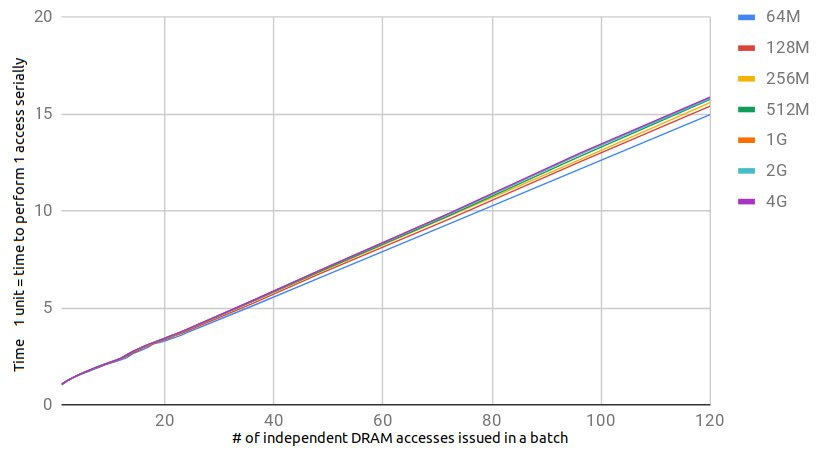
\includegraphics[width=\linewidth]{equivalentCost.png}
%  \caption{equivalentcost}\label{fig:equivalentcost}
\endminipage\hfill
\minipage{0.50\textwidth}
  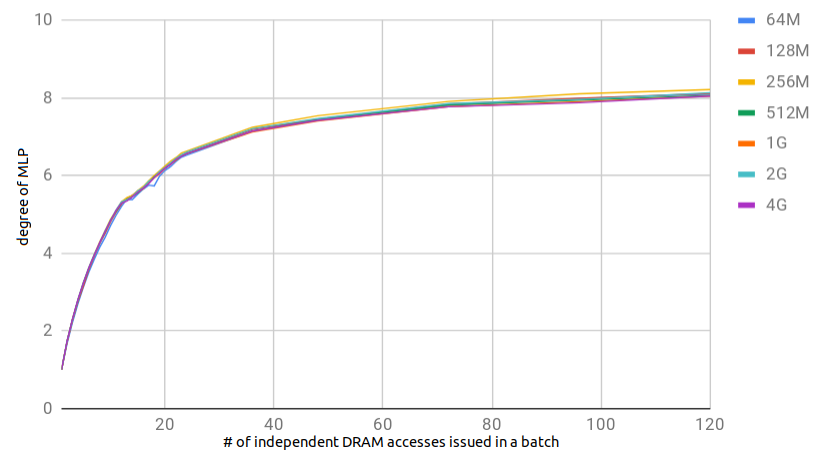
\includegraphics[width=\linewidth]{equivalentMLP.png}
%  \caption{equivalentmlp}\label{fig:equivalentmlp}
\endminipage\hfill
\caption{Left: the time it takes to complete $K$ independent accesses in parallel, 
normalized against the time it takes to complete $1$ access. 
Right: the equivalent memory level parallelism degree one can reach by issuing down $K$ accesses at a time. 
Colors: different sizes of array $arr$.}
\label{mlprealworld}
\end{figure}

As shown in Figure \ref{mlprealworld}, the time it takes to perform $K$ independent accesses in parallel 
is pretty much linear with respect to $K$. 
One can obtain the following empirical formula from the figure, to characterize the 
time it takes to perform $K$ independent parallel accesses in terms of $T$, the equivalent number of serial accesses:
\begin{center}
$T=1+c\cdot (K-1)$
\end{center}
where $c$ is a constant that depend on the specific hardware. 
In Figure \ref{mlprealworld}, measured on the \textit{Skylake} laptop, $c\approx 0.117$. 
The \textit{Haswell} multi-socket server also has $c\approx 0.117$, 
while the AMD \textit{Epyc} multi-socket server has $c\approx 0.065$,
which suggests that AMD CPUs can track more outstanding DRAM accesses in parallel than Intel can. 

\subsection{The Effect of Adjacent-Line Prefetcher} \label{adjlineprefetcher}

In this section, we measure the performance of a particular hardware prefetcher -- the adjacent-line prefetcher. 
When one accesses a cache line, the adjacent-line prefetcher will automatically prefetch 
its ``adjacent cache line'', the cache line that complements the accessed cache line in its 128-byte block, 
into the CPU cache. 

To measure the effect of adjacent-line prefetcher, one needs to construct a code snippet 
that accesses the adjacent line of a previously accessed line. 
However, one must ``hide'' the address of that access from speculative execution mechanism, 
to make sure that we are measuring the effect of hardware prefetcher, not speculative execution. 
This can be done via the following trick: 
access a few (say 8) random cache lines first, and accumulates the results. 
We then access the adjacent cache line of the $k$-th access, where $k$ is the residue of the accumulator modulo 8. 
We are always accessing an adjacent line, 
but which line to access is not known until all prior DRAM accesses have completed.
So the best thing speculative execution can do is blindly guess the residue, 
which is unlikely to hit since there are 8 possibilities. 

We also measured two other interesting cases: 
change the adjacent line access to instead access the cache line itself (which will be a L1 hit), 
and access the ``non-complementary'' adjacent line, which is the line adjacent to the cache line, 
but resides in the other 128-byte block.

Suppose a DRAM access takes 1 unit of time. 
Experiments showed that an L1-hit takes around 0.1 unit of time, 
the adjacent line access takes around 0.2 unit of time, 
and the ``non-complementary'' adjacent line, somewhat surprisingly, takes 1 unit of time.

This suggests that the hardware adjacent-line prefetcher indeed allows 
the programmers to access the adjacent line at a relatively low cost (only twice the cost of an L1-hit). 
However, it is important that one aligns its 128-byte block of data along the 128-byte boundary. 
If one mistakenly aligned the block along a 64-byte boundary that is not a 128-byte boundary,
the access to the ``adjacent line'' will take the full cost of 1 DRAM access time. 

\subsection{Tricks for Minimal Latency} \label{misctricks}

We note that a few tricks are needed for best results of memory level parallelism. 
The most important trick is to enable huge pages. 
For random accesses over a huge address range, 
it is likely that every access is a TLB miss if the default 4KB pages are used. 
This turns out to have a very significant impact on the potential of memory level parallelism. 
Figure \ref{mlp_4kb} is the result of the experiment in Section \ref{mlpmeasurement}, 
except that the 4KB page is used instead of 1GB huge page. 

\begin{figure}[!htb]
\minipage{0.50\textwidth}
  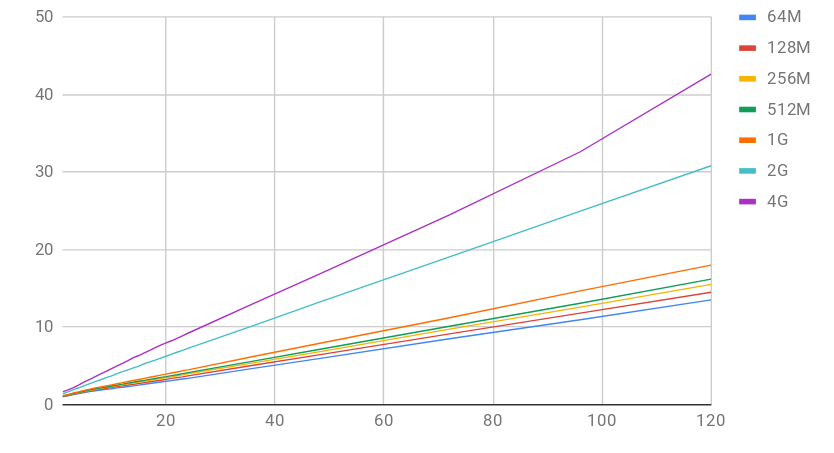
\includegraphics[width=\linewidth]{equivalentCost_4k.png}
%  \caption{equivalentcost}\label{fig:equivalentcost}
\endminipage\hfill
\minipage{0.50\textwidth}
  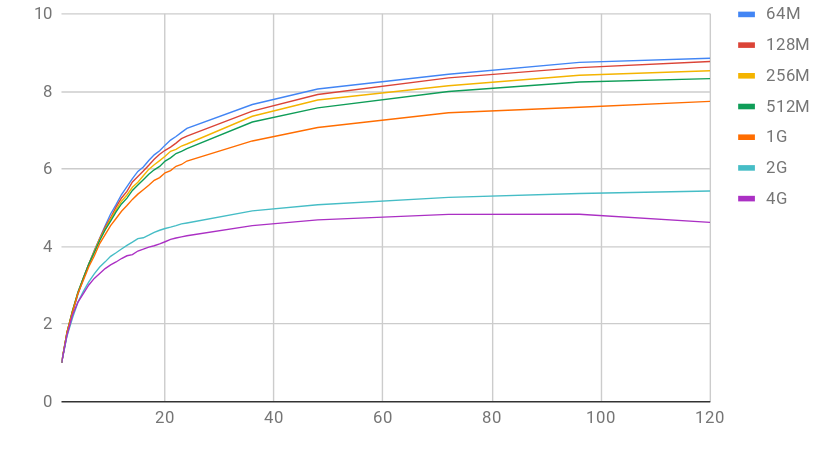
\includegraphics[width=\linewidth]{equivalentMLP_4k.png}
%  \caption{equivalentmlp}\label{fig:equivalentmlp}
\endminipage\hfill
\caption{Experiment of Figure \ref{mlprealworld}, but run with default 4KB pages.}
\label{mlp_4kb}
\end{figure}

As one can see, the performance quickly degenerates as the array size becomes larger. 
On 4GB array, we could only achieve MLP slightly over 4, compared with 8 in the 1GB page case. 
2MB huge page turns out to be sufficient as well: it is slower than 1GB pages, but only slightly.

Multi-socket servers may need additional tricks for optimal performance.
First, the thread should be pinned to a fixed CPU, as otherwise it may be migrated to another socket 
by the kernel, then all DRAM accesses would be on the other NUMA node, which will be significantly slower. 
Second, due to cache coherency issues, every access to DRAM needs to consult the caches of the other CPU socket, 
to make sure it is not concurrently modified by the other CPU socket. 
However, if the other CPU socket is idle, it will run at a much lower frequency, 
which will make answering those cache coherency requests slower. 
So one should run an infinite loop on the other CPU socket to keep it busy and run at full frequency. 

Filling more DRAM slots on the motherboard is also helpful for best performance. 
All plots presented above are run with only 1 DRAM chip, 
leaving the 3 other slots on the motherboard empty.
If one plugs in 2 DRAM chips, one can actually get $\sim$10\% better results in high MLP cases.
This might be caused by contention on the DRAM chip when MLP is high.

\section{Lock-free Skiplist Iterator} \label{sliter}

Lock-free skiplist is a popular choice of index data structure for main memory databases.
One of its most important use cases is to support range query: 
given a range on the index key, one wants to iterate through every item which index falls in the range in increasing order.
There are often at least hundreds of items falling in the specified range.
In that case, iterating through every item in the range will take the majority of the time, 
compared with the $O(\log n)$ time to find the boundary nodes corresponding to the ranges.
Unless the keys are inserted in increasing order, it is clear that every iteration will be a cache miss.

In this section, we describe how to speed up this iteration process. 
Our iterator provides the identical API as the plain iterator 
-- specifically, the ``++()'' method that advances the iterator to the next node,
and plain pointer dereference to access the current node.
This makes us a drop-in replacement of the plain iterator for higher-level applications.
In Section \ref{sliter_singlethread}, 
we elaborate the idea on a single-threaded skiplist, 
and demonstrate a 4x speed-up. 
In Section \ref{sliter_memsql}, 
we extend our iterator to support lock-free versioned skiplist, 
and integrated our iterator into MemSQL \cite{memsql}, a commercial main memory database, 
and evaluated the performance impact on real SQL queries. 
We demonstrated that our iterator results in 1.9x end-to-end query time speedup when there is only one query thread. 
With multiple query threads, we still achieve 1.5x to 1.9x speedup.

\subsection{Single-threaded Skiplist Case} \label{sliter_singlethread}

We first briefly review how skiplist works. 
A skiplist is essentially a multi-layer linked list. 
The bottom-most (0th) layer is a linked list of all items, in sorted order. 
For each $k\geq 0$, layer $k+1$ is a linked list of a subset of items in layer $k$, 
sampled with a probability of $1/2$, in sorted order. 
This results in a so-called skiplist tower, as shown in Figure \ref{skiplist_tower}.
 
\begin{figure}[!htb]
  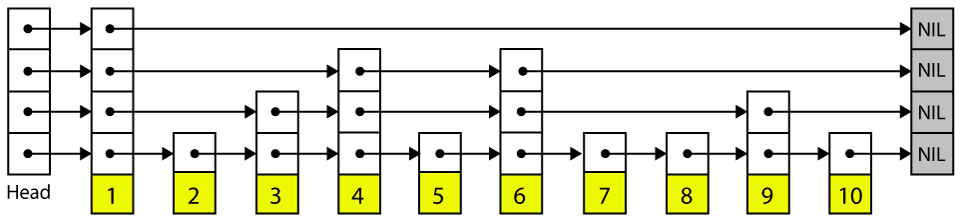
\includegraphics[width=\linewidth]{skiplistTower.png}
\caption{An illustration of a skiplist tower, from \cite{memsqladamblog}}
\label{skiplist_tower}
\end{figure}

Since each layer is a sampling of its next layer with probability $1/2$, 
there are $O(\log n)$ layers in expectation for a skiplist containing $n$ items, 
and there are expected $O(1)$ items in the next layer between two adjacent nodes of any layer. 
This allows one to answer a $\lowerbound$ query in expected $O(\log n)$ time by traversing from the start of top layer, 
moving along the linked list as long as the next node is smaller than the given bound, 
and moving down to the next layer when the condition is not satisfied. 
After the two boundary nodes corresponding to the specified range are found, 
iterating through every node in this range is no different from iterating a linked-list: 
one simply traverse along the bottom-most layer starting from the left boundary node, until the right boundary node is reached.
While the data structure is very straight-forward, for clarity, 
we still provide the prototype of the skiplist as well as a plain iterator:

\singlespacing\begin{codebox}
\begin{minted}{c++}
struct Node {
    // the payload, which we don't care
    PayloadType payload;
    // height of tower of this node 
    int height;	
    // an array of length height, next[k] is next node in layer k
    Node* next[]; 
};
\end{minted}
\end{codebox}\doublespacing

\singlespacing\begin{codebox}
\begin{minted}{c++}
struct Iterator {
    Node* current;
    // Access current position
    Node& operator*() { return *current; }
    // Advance to next position
    Iterator& operator++() { 
        // Move to next node along bottom-most linked-list 
        current = current->next[0]; 
        return *this;
    }
};
\end{minted}
\end{codebox}\doublespacing

Interestingly, one can easily show that it is impossible to leverage MLP 
from linked-list iteration: the address of current\verb|->|next\verb|->|next will not be known, 
until current\verb|->|next is fetched from memory. 
This is exactly the ``worst case'' in Section \ref{specexec} where each access (directly or indirectly) depends on every access before it, 
so the plain iterator has MLP=1.

How could we get more MLP? 
The trick is, the skiplist tower gives us a way to know about nodes further ahead: 
current\verb|->|next[k] will give us a node approximately $2^k$ steps away from current node.
Of course, this only works if the tower height of current is at least $k$.

So a natural idea to issue down more than one independent accesses at once is to use the level 1 tower. 
Whenever we encounter a node $c$ with height larger than 0 (which happens with 50\% probability), we will prefetch c\verb|->|next[1]. 
If c\verb|->|next[1] is not equal to c\verb|->|next[0] (which happens with 50\% probability), 
then we prefetched something useful. This allows us to have MLP=2 with 25\% probability, and MLP=1 otherwise, 
resulting in an overall MLP of 1.25, as shown below.

\singlespacing\begin{codebox}
\begin{minted}{c++}
// Naive prefetch strategy using level 1 tower
Iterator& operator++() { 
    // Prefetch level 1 tower if useful
    if (height > 0 && current->next[0] != current->next[1]) {
        __builtin_prefetch(current->next[1]);
    }
    // Move to next node along bottom-most linked-list 
    current = current->next[0]; 
    return *this;
}
\end{minted}
\end{codebox}\doublespacing

We can extend the idea to do better by using the higher tower levels as well. 
We will have a queue of ``prefetch tasks'', each described by a triplet $(start,end,level)$. 
The triplet means that $start$ has been prefetched to cache (so accessing $start$.next[] will not be cache-missing), 
we want to prefetch everything between $start$ and $end$,
and the highest layer linked-list that connects $start$ and $end$ is $level$. 
To process such a task while maintaining the invariant, we will: 
\begin{itemize}
[topsep=0pt,partopsep=0pt,itemsep=0pt,parsep=0pt,fullwidth,itemindent=\parindent,listparindent=\parindent]
\item Prefetch $start$.next[$i$] for each $0\leq i\leq level$.
\item Add a task to traverse from $start$.next[$i$] to $start$.next[$i+1$] via level $i$, for $0\leq i<level$.
\item Add a task to traverse from $start$.next[$level$] to $end$ via $level$.
\end{itemize}

This gives us the following pseudo-code:

\singlespacing\begin{codebox}
\begin{minted}{c++}
struct QueueItem {
    Node* start; Node* end; int level;
};
// Process a prefetch task, and enqueue generated tasks into q
void ProcessQueueItem(QueueItem task, queue<QueueItem>& q) {
    // Step 0: check termination case
    if (task.start == task.end) {
        return;
    }
    Node* n = task.start;
    // Step 1: prefetch next node in each layer
    for (int i = 0; i <= task.level; i++) {
        __builtin_prefetch(n->next[i]);
    }
    // Step 2 & 3: put generated tasks into q
    for (int i = 0; i < task.level; i++) {
        q.Push(QueueItem(n->next[i], n->next[i+1], i));
    }
    q.Push(QueueItem(n->next[level], task.end, task.level));
}
// Process a whole queue of tasks, returns new queue of tasks
// Note that all accesses in this function are cache-resident,
// and all prefetches are independent and executed in parallel
void ProcessQueue(queue<QueueItem>& q) {
    queue<QueueItem> newQueue;
    while (!q.Empty()) {
        ProcessQueueItem(q.Pop(), newQueue);
    }
    q = newQueue;
}	
\end{minted}
\end{codebox}\doublespacing

Analyzing the code above, it is not hard to see that for a task with level $k$, 
it will be fully ``digested'' in $k$ steps, 
while producing on expectation $C_k^i$ non-empty ($start\neq end$) items in the $i^{th}$ step. 
So if we push a new level $K$ task into the queue in every phase, 
the queue will stabilize at expected $1+\sum_{i=1}^K C_K^i=2^K$ items, 
with expected $2^K$ useful prefetches issued in parallel in each phase.
This allows us to reach an arbitrary degree of memory level parallelism in theory by picking a large enough $K$.
In practice, $K=3$ or $4$ yields the best results, 
which is a result of balance between larger constants hidden in the algorithm and higher MLP, 
and the fact that Intel CPUs can in theory have a maximal MLP of 10.
The pseudocode can be found below.

\singlespacing\begin{codebox}
\begin{minted}{c++}
// Max tower level to be used 
const int K = 3;
struct Iterator {
    Node* current;
    // The prefetch queue, size 2^K on expectation
    queue<QueueItem> q;
    // The furthest node reached and prefetched
    // It must be a node of height at least K
    Node* furthest;
    // Issue one phase of prefetches
    // On expectation 2^K parallel prefetches will be issued
    void Prefetch() {
        // Process each item in the queue 
        ProcessQueue(q);
        // Finally add a new level K task into queue
        q.Enqueue(QueueItem(furthest, furthest->next[K], K));
        // Advance and prefetch furthest node
        furthest = furthest->next[K];
        __builtin_prefetch(furthest);
    }
    // Advance iterator
    Iterator& operator++() {
        // Start a new phase of prefetching when needed
        while (current == q.Head().start) {
            Prefetch();
        }
        // Move to next node along bottom-most linked-list 
        current = current->next[0]; 
        return *this;
    }
    // Setup prefetch queue on construction 
    Iterator(Node* current) : current(current) {
        // Find the first node n with height >= K by brute force
        Node* n = ....
        // Setup prefetch queue and the "furthest" node
        q.Push(QueueItem(n, n->next[K], K));
        furthest = n->next[K];
        __builtin_prefetch(furthest);
    }
}
\end{minted}
\end{codebox}\doublespacing

We benchmarked this improved iterator against the plain iterator. 
Experiments showed that for long iterations of a few hundred items, 
we are 4x faster than the plain iterator.
Since our iterator has a ramp-up cost (we need to find a node with at least tower level 3, 
and for the first few phases our queue is not having the full expected size thus less MLP, 
and for the last few phases we may prefetch items that are outside range), 
for short iterations our advantage is smaller. 
However, we are advantageous as long as the range contains at least around 20 items.

\subsection{Evaluation in MemSQL, a Real World Database} \label{sliter_memsql}

In this section, we demonstrate the performance impact of our iterator in MemSQL \cite{memsql}, 
a commercial main memory database.
The benchmark is run on the personal laptop, 
with hardware setting Intel Core i7-7700HQ CPU at 2.80GHz and 1x16GB Corsair DDR4 2400MT DRAM.

MemSQL uses a versioned lock-free skiplist as their in-memory index, with each node represent a row of data. 
Versioning is necessary to support snapshot isolation.
Specifically, each lock-free skiplist node stores a lock-free linked-list of all versions of the data in that row.
To find the row that correspond to a specific snapshot version,
one needs to iterate the linked-list to find the largest version that is smaller than the given snapshot version. 
So we need to prefetch not only the next nodes, but also the head of the version linked-list of the current node.
There is no optimistic locking protocol: updates are supposed to be sparse. 
As such, it is plausible to assume that most of the time the version linked-list will only contain one element, 
so we only prefetch the head of the linked list and not the deeper nodes. 

Lock-freedom is generally not a problem for us: 
lockfree skiplist implementation guarantees that 
at any point each layer is always a valid linked list even in the presence of deletes, 
and the memory are reclaimed using epochs, 
so the references we hold will also remain valid all the time. 
There is only one issue with delete: the ``\verb|while (current == q.Head().start)|'' line in advance iterator 
may never be true, if the q.Head().start were physically in the skiplist when it was pushed into queue, 
but deleted and physically removed from the skiplist by concurrent threads later. 
The solution is to instead simply execute the prefetch phase every $2^K$ advances. 
While this is less ``intelligent'' than the single-threaded version 
because we are no longer ``adapting'' to the actual tower, nonetheless it works.

We replaced the original iterator (which is just the plain iterator) in MemSQL with our iterator. 
To remove unnecessary overhead from distributed system, 
the benchmark is done under the internal SingleBox mode where all sharding and replication components are disabled.
We benchmark the performance impact of our iterator with the following table schema:

\singlespacing\begin{codebox}
\begin{minted}{sql}
CREATE TABLE t (a INT, b CHAR(16), KEY(a));
\end{minted}
\end{codebox}\doublespacing

We populate 20 million rows of random data into the table, and time the following SQL query:

\singlespacing\begin{codebox}
\begin{minted}{sql}
SELECT COUNT(*) FROM t WHERE a > @
\end{minted}
\end{codebox}\doublespacing

This allows us to compute the number of rows iterated per second. 
The original MemSQL could scan 5.0M rows per second. 
After switching to our improved iterator, we are capable of scanning 9.6M rows per second, a 1.92x speedup. 
We also tested the case of 4/8 concurrent query threads working on 2/4 available CPUs, 
the results are in Table \ref{sliter_memsql_mt}. As one can see, we achieve 1.54x to 1.93x speedup in multi-threaded cases.
 
 \begin{table}[!htb]
 \centering
\begin{tabular}{|c|c|c|c|c|c|c|}
\hline
\# Query Threads & \multicolumn{3}{c|}{2 Threads}              & \multicolumn{3}{c|}{4 Threads}              \\ \hline
\# CPUs for MemSQL       & Before      & After       & Speedup & Before      & After       & Speedup \\ \hline
2 CPUs & 19.8 & 30.5 & 54\%    & 16.8 & 27.7 & 65\%    \\ \hline
4 CPUs & 12.0 & 23.2 & 93\%    & 12.8 & 20.9 & 63\%    \\ \hline
\end{tabular}
\caption{Total throughput for multi-threaded cases in million rows per second.}
\label{sliter_memsql_mt}
\end{table}

The reason that the speedup is smaller compared with the single-threaded case may come from a few factors. 
First, the versioned lock-free skiplist contains significantly more logic than the single-threaded skiplist. 
We cannot speed up those logic, and furthermore, some of the logic contain DRAM access (for example, 
reading the version linked-list), which consumes some of the fixed hardware-available memory parallelism degree. 
Second, versioned lock-free skiplist contains a lot of memory barriers. 
Those barriers could require flushing the CPU load/store queues, which limits the memory level parallelism. 
Finally, MemSQL did not use huge pages. 
As shown in Section \ref{misctricks}, this has a negative impact on the performance of memory level parallelism.

\section{Ordered Index} \label{orderedindex}

In this section, we present $\MlpIndex$, an ordered index structure analogous to std::set.
Specifically, it supports three operations with identical APIs as std::set, namely
$\insertion$ (insert an element into the set), $\lookup$ (query if an element exists in the set) 
and $\lowerbound$ (find the minimum element in the set no smaller than the given element).
$\MlpIndex$ is not a comparison-based data structure, but an integer data structure that operates on a key universe $[0,M)$.
While our implementation currently only supports 64-bit keys ($M=2^{64}$), it could be extended to support any string keys as well.

$\MlpIndex$ takes a ``MLP-degree'' parameter $D$, 
which represents the capability of the hardware to track parallel DRAM requests, 
analogous to that B-tree takes a ``block size'' parameter that characterizes the granularity of each disk read by the hardware.
Under the assumption that $D$ independent parallel DRAM requests where each request touches one cache line can be completed in one roundtrip,
$\MlpIndex$ takes $O(\log_D\log M)$ DRAM roundtrips (which is the dominating factor of time in practice) 
and $O(D\cdot\log_D\log M)$ CPU work to execute an $\insertion$, $\lookup$ or $\lowerbound$,
and has a memory consumption of $O(n\cdot \log_D\log M)$.
If we have SIMD support on $D$-vectorized operations (specifically, arithmetic and $\simdgather$/$\simdscatter$ operation), 
the CPU work could be reduced to $O(\log_D\log M)$ as well.

To the best of our knowledge, $\MlpIndex$ is practically the fastest ordered index. 
Compared with Height Optimized Trie (HOT) \cite{hot_sigmod18}, 
the fastest state-of-the-art ordered index we are aware of, 
$\MlpIndex$ is 3x to 4x faster on $\insertion$ and $\lookup$, 
and 2x faster on $\lowerbound$.
Compared with Adaptive Radix Tree (ART) \cite{arttrie_icde13}, $\MlpIndex$ is 4x to 4.5x faster. 
On a data set of 80 million 64-bit keys, single-threaded $\MlpIndex$ only takes around 2 DRAM roundtrip time to perform 
an $\insertion$ or $\lookup$, and around 3 DRAM roundtrip time to perform an $\lowerbound$.
We note that since the data set cannot fit into cache, 
it is impossible for any algorithm to support the operations in less than the time of 1 DRAM roundtrip.
Our superior speed 
comes from a combination of algorithm-level designs to leverage memory level parallelism, 
and various engineering-level optimizations including a specially-modified hash table scheme, 
and adaptively choosing different data structures for high-degree and low-degree nodes 
to minimize the constants hidden in the algorithm.
For 64-bit keys, our algorithm only makes 6 parallel hash table lookups, 
which boil down to at most 12 independent parallel DRAM accesses in our implementation,
to execute a $\lookup$ query. $\lowerbound$ requires only one additional DRAM access
depending on the lookup results. 
$\insertion$ only writes to cache-resident addresses after the lookup 
if there is no hash table movement due to conflict.

$\MlpIndex$ is also optimal from a complexity theoretical view: as proven in \cite{ajtai88comb-lowerbound}, 
under word-RAM model and plausible assumptions on the size of the data structure, 
$\Omega(\log \log M)$ per operation is the lower bound in time to support both $\insertion$ and $\lowerbound$ operation. 

For use cases that requires both $\lookup$ and $\lowerbound$, 
a common strategy is to build a stand-alone hash table to support $O(1)$ $\lookup$, 
in addition to the ordered index that supports $\lowerbound$, 
since the native $\lookup$ operation in ordered index can be much slower than a hash table.
This strategy is applied in industrial in-memory storage engines like Redis \cite{redis}.
However, it is unnecessary for us to build the stand-alone hash table at the cost of slower $\insertion$ and extra memory, 
because in practice our native $O(\log_D\log M)$ $\lookup$ is already almost as fast as a carefully-engineered hash table could do, 
as shown in Section \ref{mlpindex_eval}.

The core idea of $\MlpIndex$ is from x-fast trie \cite{xfast}, a data structure mostly considered in theory.
X-fast trie supports $O(\log M)$ $\insertion$ and $O(\log\log M)$ $\lowerbound$, while using $O(n\log M)$ memory.
While its $\lowerbound$ performance is theoretically optimal as proven in \cite{ajtai88comb-lowerbound},
its huge constants hidden in the algorithm as well as huge memory consumption made it not considered useful in practice. 
Indeed, the algorithm proposed in the original paper requires 64 hash table nodes to store a 64-bit key, 
and each hash table node needs to store the information of 4 pointers and 5 keys. 
That's already 4.5KB in space (550x larger than the original key size), 
and we haven't even considered the load factor of the hash table yet. 
While the authors proposed y-fast trie, 
an improvement over x-fast trie that improved the $\insertion$ performance to $O(\log\log M)$ and space consumption to $O(n)$, 
the improvement is mainly theoretical and introduces even larger constants hidden in the big-O notation. 
We are not aware of any attempts to implement x-fast trie or y-fast trie as a practically usable data structure. 

We did not use the ideas in y-fast trie. Our insertion complexity already matches that of y-fast trie, 
and while our memory consumption is worse than y-fast trie in big-O notation, 
we would like to note that the constants hidden in the big-O is much smaller.
Specifically, in practice, we use at most 96 bytes (and can be further reduced to 36 bytes) to store a 8-byte key. 
This is competitive with state-of-the-art index structures like ART \cite{arttrie_icde13} (at most 60 byte per 8 byte key) 
and Masstree \cite{masstree} ($\sim$58 bytes per 8 byte key as reported in \cite{hot_sigmod18}).
As such, we deem the use of the ideas in y-fast trie to further reduce memory as possible but unnecessary.

In Section \ref{intro_xfast}, we briefly introduce the original idea of x-fast trie from \cite{xfast}. 
In Section \ref{mlpindex_simple} and \ref{mlpindex}, 
we elaborate the algorithm-level and engineering-level re-designs on the original idea that leads to $\MlpIndex$, 
and in Section \ref{mlpindex_eval} we benchmark the performance against a few state-of-the-art ordered index implementations. 

\subsection{Original x-fast Trie Idea} \label{intro_xfast}

X-fast trie assumes that all keys have a length of $\log M$ bits.
In its essence, a x-fast trie is a plain binary trie that carries a few extra information on the node:
\begin{itemize}
[topsep=0pt,partopsep=0pt,itemsep=0pt,parsep=0pt,fullwidth,itemindent=\parindent,listparindent=\parindent]
\item Prefix: the prefix that this node represents in the trie.
\item Min/Max: records the leaf corresponding to minimum/maximum key in this subtree.
\item Prev/Succ: if the node is a leaf, records the prev/succ leaf (the ``leaf-link'').
\end{itemize}

\singlespacing\begin{codebox}
\begin{minted}{c++}
// A Node for x-fast trie based on original idea
struct Node {
    // parent node
    Node* parent;
    // two child nodes corresponding to 0 and 1
    Node* child[2];
    // min and max leaf in this subtree
    Node *min, *max;
    // previous and successor key if this node is leaf
    Node *prev, *succ;
    // the prefix that this node represents in the trie
    Key prefix;
    // the height of this node in trie
    int height;
};
\end{minted}
\end{codebox}\doublespacing

Those information is dynamically updated using the information stored in its 0/1 children, 
for example, if one of the children of node $n$ is modified, one can update n\verb|->|min
using the logic described in the following straight-forward pseudocode:

\singlespacing\begin{codebox}
\begin{minted}{c++}
if (n->IsLeaf) {
    n->min = n;
} else if (n->child[0] != nullptr) {
    n->min = n->child[0]->min;
} else {
    n->min = n->child[1]->min;
}
\end{minted}
\end{codebox}\doublespacing

Furthermore, all the trie nodes are put into a hash table, indexed by the ``Prefix'' field of the node. 
This allows one to directly locate a node that corresponds to a given prefix in $O(1)$, without the need to walk through the path 
to that node from the root. This also allows $O(1)$ $\lookup$ 
since a $\lookup$ is simply checking whether a leaf node exists in the hash table.

The core operation of x-fast trie is $\QueryLCP$ (LCP stands for longest common prefix): 
given a key $x$, find the length of the longest prefix of $x$, 
such that the prefix corresponds to a node in the trie. The most naive way to support $\QueryLCP$ is to just 
start from the root and move down according to the bits of $x$. When a child does not exist, 
the height of the current node is the desired result. This takes $O(\log M)$ per query.

The hash table allowed us to do better. One can easily see that ``whether a prefix exists in the trie tree'' 
is monotonic with respect to the length of the prefix: suppose that the answer is $k$, 
then every prefix of length $0\leq i\leq k$ exists, but any prefix of length $i>k$ does not. 
So we can binary search on that length and query the hash table to know if a prefix exists in $O(1)$. 
This reduces the time complexity to $O(\log\log M)$. 

We can support $\lowerbound$ in $O(\log\log M)$ based on $\QueryLCP$. 
Suppose the LCP has length $k$ bits and the node of LCP is $n$. 
Since $n$ is the LCP, $n$ must not have child $x[k]$, as otherwise there will be a longer common prefix. 
However, $n$ must have child $1-x[k]$, since $n$ is the prefix of some key in the trie. 
If $x[k]=0$, then $x$ is smaller than everything in this subtree, 
so the desired lower bound of $x$ is the minimum node in this subtree (n\verb|->|min). 
If $x[k]=1$, then $x$ is larger than everything in this subtree, 
so the lower bound of $x$ is the smallest node larger than the maximum node (n\verb|->|max\verb|->|succ). 
This results in the following pseudocode:

\singlespacing\begin{codebox}
\begin{minted}{c++}
Node* Lower_Bound(Key x) {
    int len; Node* n;
    std::tie(len, n) = QueryLCP(x);
    if (len == logM) {
        // the key exists in the trie
        return n;
    }
    // x[len] represent the bit "len" of x
    if (x[len] == 0) {
        return n->min;
    } else {
        return n->max->succ;
    }
}
\end{minted}
\end{codebox}\doublespacing

Performing an $\insertion$ operation is very similar. 
After finding the LCP node $n$, one just needs to build a path of new nodes to the leaf from $n$, 
and update the extra-information fields of all the nodes from the root to the newly inserted leaf,
which takes $O(\log M)$:

\singlespacing\begin{codebox}
\begin{minted}{c++}
// Insert a key into the trie, returns if the insertion took place
bool Insert(Key x) {
    int len; Node* n;
    (len, n) = QueryLCP(x);
    if (len == logM) {
        // the key exists in the trie
        return false;
    }
    // Find the lower_bound of x, for updating leaf-link later
    Node* succ = Lower_Bound(x);
    // Construct nodes all the way to the leaf
    for (int i = len; i < logM; i++) {
        Node* newNode = new Node(....);
        n->child[x[i]] = newNode;
        hashTable.Insert(newNode);
        n = newNode;
    }
    // Update leaf-links
    n->succ = succ; n->prev = succ->prev;
    succ->prev->succ = n; succ->prev = n;
    // Update fields such as Min/Max all the way to the root
    while (n != root) {
        n = n->parent;
        UpdateFields(n);
    }
    return true;
}
\end{minted}
\end{codebox}\doublespacing

\subsection{The Core Idea of MLPIndex} \label{mlpindex_simple}

In this section, we present the two core ideas that build up the theoretical aspect of $\MlpIndex$:
\begin{itemize}
[topsep=0pt,partopsep=0pt,itemsep=0pt,parsep=0pt,fullwidth,itemindent=\parindent,listparindent=\parindent]
\item Use $D$-ary search to replace binary search in $\QueryLCP$ for high memory level parallelism.
This reduces the DRAM roundtrips required per $\lookup$ and $\lowerbound$ query from $O(\log\log M)$ to $O(\log_D\log M)$, 
with $D$ parallel requests sent in each roundtrip.
\item Support path compression (also known as ``Patricia'' \cite{patricia}) for lower insertion cost and memory consumption. 
This reduces $\insertion$ cost from $O(\log M)$ to $O(\log_D\log M)$ DRAM roundtrips and $O(D\cdot \log_D\log M)$ CPU work, 
and reduces memory consumption of the data structure from $O(n\cdot\log M)$ to $O(n\cdot\log_D\log M)$.
\end{itemize}

\subsubsection*{Using $D$-ary search}

In x-fast trie, we use a binary search to find the LCP between a given key and the set of keys in the data structure.
While theoretically optimal, it does not make use of memory level parallelism, 
since we could not know if the answer is falling in the left half or the right half of the interval, 
until the current query is complete. 
A natural modification is to use $D$-ary search instead. 
We split the current interval $[l,r]$ into $D$ parts, 
and query length $l+(r-l)/D$, $l+(r-l)/D*2$, $\cdots$, $l+(r-l)/D*(D-1)$.
The DRAM accesses from those hash table queries are independent and can be executed in parallel.
We can then narrow down to an interval that is $1/D$ size of the original.
This reduces the DRAM roundtrips required per $\lookup$ and $\lowerbound$ query from $O(\log_2\log M)$ to $O(\log_D\log M)$.

\subsubsection*{Supporting path compression}

A plain trie storing $n$ keys of length $L$ can have $O(nL)$ nodes.
Path compression is a technique that reduces the number of nodes by contracting nodes with only one child 
(except for the root node, which may only have one child). 
Any node in a path-compressed trie is either the root node, or a leaf node, or an internal node with at least 2 children. 
It is easy to see that for a path-compressed trie with $n$ leaf nodes, there are at most $n$ internal nodes, 
so a path-compressed trie of $n$ keys can have $2n$ nodes at most.

However, path compression does not work directly in x-fast trie, 
because it breaks the property that binary search relies on. 
Let's say, the original trie has a path $root\rightarrow a\rightarrow b$, 
and $a$ is removed due to path compression. 
Then one will see that prefix length $0,2$ exists in the hash table, 
but $1,3$ does not. Binary search no longer works.

To build up our intuition, we will start with an incomplete solution.
A straightforward way to workaround the unwanted interaction between path-compression and binary search
is to do an ``incomplete'' path compression instead. 
When we insert a new node at depth $k$,
we want to make sure that the $D$-ary search can narrow down correctly in each step to not miss the new node.
Therefore, for each $D$-ary search depth $d$, 
we create a intermediate node at the largest depth smaller than $k$ that search $d$ will check.
Since the $D$-ary search takes $\log_D\log M$ steps to complete, 
now we need to create at most $O(\log_D\log M)$ intermediate nodes for each new node inserted, 
so the trie may contain at most $O(n\cdot \log_D\log M)$ nodes. 
As an example, Figure \ref{intermediate_nodes} illustrates what happens when we want to insert
a new node (the red one) when $D=3$. 
We need to make sure that $D$-ary search will be able to find the new node. 
The $D$-ary search will check the nodes labeled ``1'' first. 
In order for the search to not miss our red node, we need to materialize the ``1'' node before to our newly inserted node. 
Then the search will check the two nodes labeled ``2'' in second phase, and the last two nodes labeled ``3'' in third phase,
so similarity we need to materialize the ``2'' and ``3'' node before our newly inserted node (the green nodes).

\begin{figure}[!htb]
  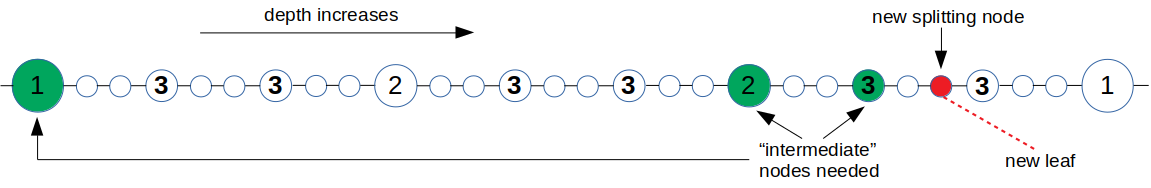
\includegraphics[width=\linewidth]{intermediate_nodes.png}
\caption{Illustration of the intermediate nodes (green nodes) needed when creating a new node (the red node), $D=3$. 
All nodes above were contracted by path compression initially.
The number on the nodes denote in which phase of $D$-ary search 
it will potentially be checked (the unlabeled nodes are potentially checked in 4-th phase).}
\label{intermediate_nodes}
\end{figure}

However, the tree resulted from the above approach can still have height $\log M$ in worst case.
Since $\insertion$ may update all the extra-information fields along the path, 
it would still result in a $\insertion$ cost of $O(\log M)$.

The solution is to employ a recursive approach. 
We build a path-compressed trie tree of depth $D$, with each node has a fan-out of $M^{1/D}$, 
so the children of a node will be values in $[0, M^{1/D})$.
We use the same data structure recursively to maintain the list of children of each node.
The special case is the root node with only one child -- 
this correspond to the ``intermediate'' nodes due to incomplete path compression, which only has one child. 
In order to achieve the memory complexity of $O(n\log_D\log M)$, 
we need to treat them specially -- since it can only happen on the root node, 
we can just store the key directly in that case. 

Note that in practice, we do not necessarily use the same data structure recursively to manage the children of a node. 
We can use different structures according to the size of the key universe. 
Specifically, in 64-bit key case, we have $D=8$ trie tree as outer-level data structure 
that results in a node fan-out of 256. 
The trie tree turns out to be too heavy-weighted to be used as the inner-level structure, 
since the key universe has a size of only 256.
We use either a list of children (if the number of children is small) 
or a bitmap to maintain the children list as our inner-level data structure. 
This is elaborated in Section \ref{mlpindex}.
 
Another question arise from path compression is how we should index our node in the hash table, 
since now each node has a ``prefix'', which is the string represented by its parent node 
plus the string represented by the edge leading to this node, 
as well as a ``path compression string'' that follows the ``prefix''. 
The string represented by this node in the trie is its ``prefix'' concatenate its path-compression string, 
as shown in Figure \ref{mlpindex_node}.

\begin{figure}[!htb]
  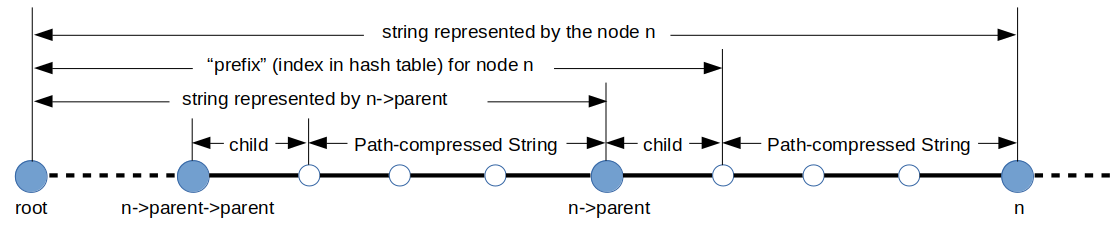
\includegraphics[width=\linewidth]{mlpindex_node.png}
\caption{Illustration of the correct way to index nodes in hash table after we apply path-compression.
Blue nodes are real nodes, hollow nodes are contracted nodes by path compression.}
\label{mlpindex_node}
\end{figure}

It turns out that we should use the ``prefix'' as a node's index 
in the hash table. This is because at the beginning of each phase of the $D$-ary search
we could only know the prefix of the node we want to lookup. 
If we use the represented string as the index, we would have a chicken and egg problem as 
there is no way to know the path-compression string corresponding to a node
until we locate that node in the hash table, which we can't because we don't know the path-compression string. 
This leads to a node prototype as shown in the pseudocode below.
Figure \ref{mlpindex_structure_illustration} illustrates the recursive structure of \MlpIndex, 
as well as how the pointers defined in the pseudocode points to each other.

\singlespacing\begin{codebox}
\begin{minted}{c++}
struct Node {
    // The length of key in bits for this key universe
    int len;
    // The index into the hash table
    Key prefix;
    // The string represented by this node
    // which is prefix + path-compressed string
    Key fullKey;
    // The hash table storing all nodes in this DS
    HashTable* hashTable;
    // Additional information as in original x-fast trie
    // Min and max node in this subtree 
    Node* min, max;
    // Leaf-links if this node is a leaf
    Node* prev, succ;
    // Whether or not this is a special ``intermediate node''
    // if it is, then it must be the root of its parent DS,
    // and fullKey is the only key stored in this DS
    bool isSpecialIntermediateNode;
    // A recursive DS to manage the children of this node,
    // which works on a key universe of length len / D bits
    Node* children;
    // The parent DS of this DS, 
    // which works on a key universe of length len * D bits
    Node* parent;
};
\end{minted}
\end{codebox}\doublespacing

\begin{figure}[!htb]
  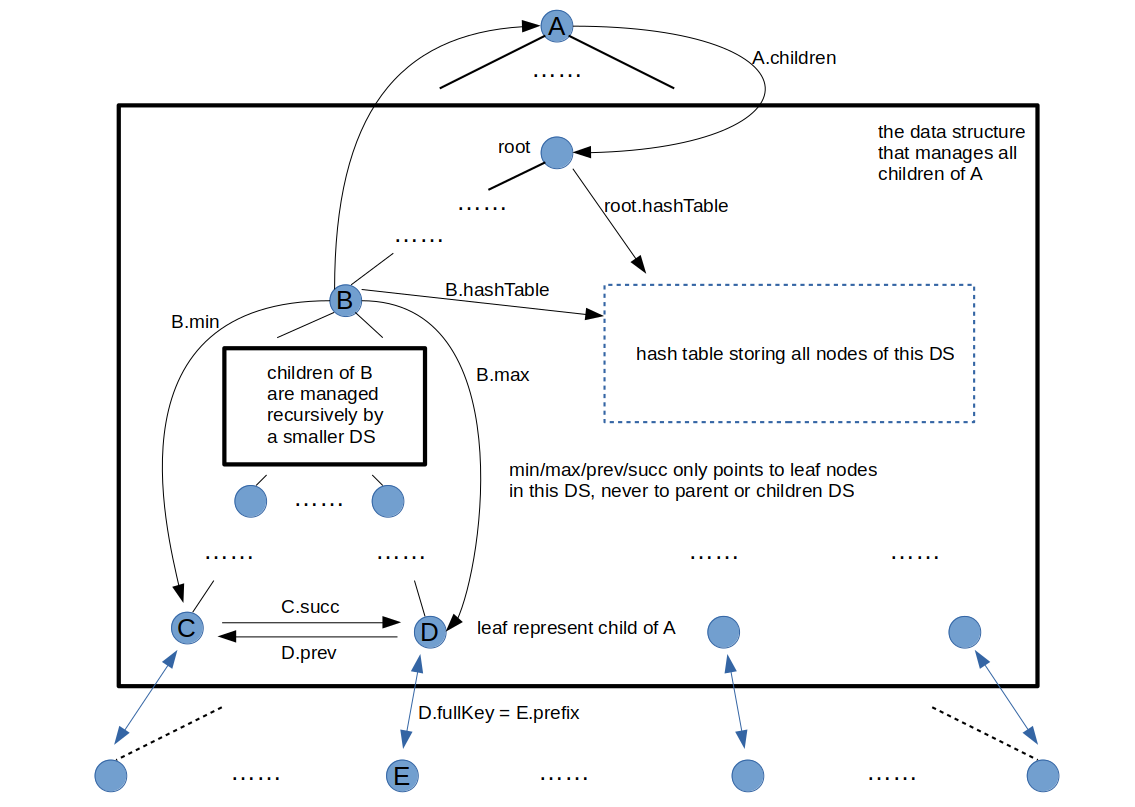
\includegraphics[width=\linewidth]{mlpindex_structure_illustration.png}
\caption{Illustration of the recursive structure of \MlpIndex.}
\label{mlpindex_structure_illustration}
\end{figure}

To find the LCP, we simply query all the $D$ levels of the trie. 
Since we query every depth, path-compression is not a issue for us.
After we find the LCP node $n$ in this trie, we first check if the path-compression string matches. 
If not, then $n$ is the LCP node and we can return. Otherwise, 
we need to recurse to the children of $n$ to find the LCP inside the children of $n$. 
In each step we query $D$ independent hash table positions, and the recurse ends in $O(\log_D\log M)$ steps, 
resulting in a complexity of $O(\log_D\log M)$ DRAM roundtrips and $O(D\cdot\log_D\log M)$ CPU work,
as shown below (in which it assumes for simplicity that the length of key is a power of $D$).

\singlespacing\begin{codebox}
\begin{minted}{c++}
// Recursive QueryLCP on path-compressed trie
// t is the root of the data structure that 
// stores the bits [currentDepth, currentDepth + t->len) of 
// all keys starting with bits x[0:currentDepth)
// Returns the LCP node n, 
// the length of LCP is lcp(n->fullKey, x)
Node* QueryLCP(Node* t, Key x, int currentDepth) {
    // termination case (reached last level):
    if (t->len == 1) {
        return t;
    }
    // termination case (intermediate node):
    if (t.isSpecialIntermediateNode) {
        return t;
    }
    Node* lcpNode = t;
    // Query every depth of the trie to find LCP
    // Those queries are independent and the DRAM accesses 
    // from these queries are executed in parallel
    int step = t->len / D;
    for (int i = 1; i < D; i++) {
        int len = i * step;
        // substring [0, currentDepth+len) of x
        Key prefixToFind = x[0:currentDepth+len];
        Node* n = t->hashTable.Find(prefixToFind);
        if (n != nullptr) {
            lcpNode = n;
        } 
    }
    // The length of the string represented by lcpNode
    int fullKeyLen = lcpNode->fullKey.length();
    // If the path-compression string does not fully match 
    // corresponding parts in x, then it's already over
    // and no need to recurse into child
    if (x[0:fullKeyLen] != lcpNode->fullKey) {
        return lcpNode;
    }
    // The LCP falls in range [fullKeyLen, fullKeyLen + step)
    // Recurse to the child DS of that node to find it
    return QueryLCP(lcpNode->children, x, fullKeyLen);
}
\end{minted}
\end{codebox}\doublespacing

$\lookup$ operation can be built directly upon $\QueryLCP$, 
since all we need to check is whether n\verb|->|fullKey is exactly the key we are looking for, 
where n is the LCP node.
However, note that it is incorrect to simply query if $x$ exists in root\verb|->|hashTable, 
since the index in the hash table does not include the path-compression string part.
The pseudocode can be found below.

\singlespacing\begin{codebox}
\begin{minted}{c++}
// Returns whether key x exists in the data structure
bool Lookup(Node* root, Key x) {
    Node* n = QueryLCP(root, x, 0 /*currentDepth*/);
    return n->fullKey == x;
}
\end{minted}
\end{codebox}\doublespacing

$\lowerbound$ operation can also be supported in $O(\log_D\log M)$ by $\QueryLCP$ and the extra information 
carried on the node, using identical idea as the original x-fast trie. 
There are only two complications compared with the original x-fast trie: 
first, we need to handle the case that the path-compression string does not match; 
second, that the children of a node is managed by a recursive data structure, 
so we need to find the $\lowerbound$ of the LCP string first, 
by finding the lower bound among the children if possible, 
and going upward to the parent data structure if the lower bound does not exist in children.
After we find the $\lowerbound$ of the LCP string, 
the real $\lowerbound$ is the smallest string starting with the LCP string, 
which can also be found by going upward the parent data structure.
The pseudocode can be found below:

\singlespacing\begin{codebox}
\begin{minted}{c++}
// Returns the minimum key no smaller than key x
Key Lower_Bound(Node* root, Key x) {
    Node* n = QueryLCP(root, x, 0 /*currentDepth*/);
    // Recall that the property of LCP node is that 
    // everything in the subtree is either all smaller, 
    // or all bigger than key x
    bool isAllSmallerThanKey;
    int fullKeyLen = n->fullKey.length();
    if (n->fullKey != x[0:fullKeyLen]) {
        // If path-compression string does not match
        isAllSmallerThanKey = (n->fullKey < x[0:fullKeyLen]);
    } else {
        // path-compression string matches, 
        // then n being LCP node implies that all children 
        // must start with bit k, and x starts with bit 1-k
        isAllSmallerThanKey = (x[fullKeyLen] == 1);
    }
    // Find the lower bound of node n, 
    // using the same idea as in x-fast trie
    if (isAllSmallerThanKey) {
        while (n->max->succ == nullptr) {
            // this child is largest among the children
            // we have to move backward to its parent DS
            n = n->parent;
        }
        n = n->max->succ;
    } else {
        n = n->min;
    }
    // The answer is the smallest key with n->fullKey as prefix
    while (n->parent) {
        // Invariant: n is the leaf node in its DS,
        // so this must correspond to a node in its parent DS
        // Locate it by probing the hash table of the parent DS
        n = n->parent->hashTable.Find(n->fullKey);
        // We are now in the parent DS, 
        // move to the min node in this subtree 
        n = n->min;
    }
    return n->fullKey;
}
\end{minted}
\end{codebox}\doublespacing

Inserting into the data structure is conceptually very similar to how one inserts into a conventional 
path-compressed trie.
The only difference is that in our case the children of a node are managed by a recursive data structure. 
One first insert the ``splitting point'' node if it were a contracted node before,  
then insert the key as a new child of the splitting point node, 
which is recursively inserting into the sub-data-structure that manages the children of the splitting point, 
as shown in Figure \ref{mlpindex_insert}.

\begin{figure}[!htb]
  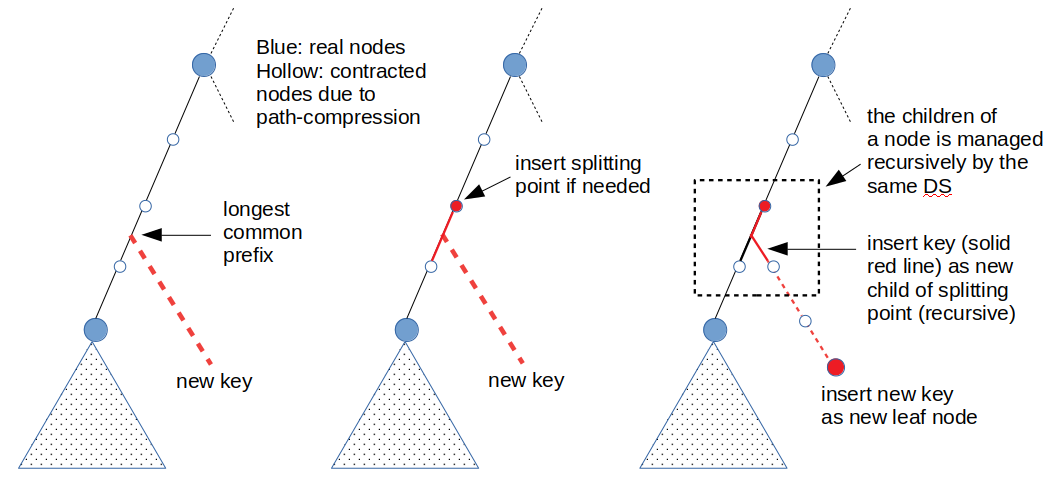
\includegraphics[width=\linewidth]{mlpindex_insert.png}
\caption{Illustration of inserting a key into $\MlpIndex$}
\label{mlpindex_insert}
\end{figure}

We additionally note that, if we apply this idea with $D=2$ as in original x-fast trie, 
the data structure can be viewed as a special form of van Emde Boas tree \cite{vebtree} with a per-node hash table.
The ``path-compression'' serves exact purpose as the trick in van Emde Boas tree that stores the ``max node'' separately, 
so only buckets containing at least 2 elements will build a sub-data-structure 
(or in the language of path compression, non-root nodes with only 1 child are contracted, 
and root node with only 1 child are specially treated), 
So from a theoretical aspect, $\MlpIndex$ can also be viewed as a hybridization of x-fast trie and van Emde Boas tree.
We summarize the theoretical complexity of relevant data structures in Table \ref{ordered_index_theoretical_comparison}.

\begin{table}[!htb]
\centering
\begin{tabular}{|c|c|c|c|c|c|}
\hline
              & x-fast          & y-fast          & vEB + HT & \begin{tabular}[c]{@{}c@{}}$\MlpIndex$\\ (No SIMD/MLP)\end{tabular}            & $\MlpIndex$ \\ \hline
$\insertion$  & $O(\log M)$     & $O(\log\log M)$ & $O(\log\log M)$ & $O(D\cdot\log_D\log M)$ & \textcolor{red}{$O(\log_D\log M)$}  \\ \hline
$\lowerbound$ & $O(\log\log M)$ & $O(\log\log M)$ & $O(\log\log M)$ & $O(D\cdot\log_D\log M)$ & \textcolor{red}{$O(\log_D\log M)$}  \\ \hline
Memory  & $O(n\log M)$     & \textcolor{red}{$O(n)$}          & $O(n\log\log M)$ & $O(n\log_D\log M)$       & $O(n\log_D\log M)$  \\ \hline
\end{tabular}
\caption{Comparison on theoretical complexity of relevant data structures.
The $\MlpIndex$ column assumes that $D$ independent DRAM requests can be completed in one DRAM roundtrip, 
and $D$-vectorized SIMD instructions are available.}
\label{ordered_index_theoretical_comparison}
\end{table}

\subsection{The Fully-Fledged MLPIndex} \label{mlpindex}

In this section, we present the ideas and tricks that are important to make $\MlpIndex$ 
extremely fast in practice. While the ideas are generally applicable, 
we focus our examples on 64-bit key case, which is the case that we benchmark in Section \ref{mlpindex_eval}.

\subsubsection*{Cuckoo Hashing}

The bottleneck of $\MlpIndex$ is the parallel hash table lookups.
Specifically, the longest probe chain of the $D$ parallel lookups determines the number 
of DRAM roundtrips needed to complete this query. 
So we want a hash table that not only optimizes the average, but also the variance of a lookup. 
Cuckoo hashing \cite{cuckoohash} turns out to be the ideal choice that achieves both goals. 
In cuckoo hashing, any existent key $x$ must exist in either position $f_1(x)$ 
or position $f_2(x)$, where $f_1$ and $f_2$ are the two independent hash functions used for the hash table.
This allows worst-case 2 DRAM accesses, and even better, all DRAM requests issued are independent. 

The original cuckoo hashing scheme allows a maximum load factor of 50\%. 
However one can improve to a load factor of 90\%+ with bucketized cuckoo \cite{bucketcuckoo}. 
Due to time limitation, we are unable to implement the bucketized cuckoo fully for $\MlpIndex$. 
However, we implemented the out-of-box experiment that 
demonstrated the memory consumption we can achieve with a modified bucketized cuckoo, 
which we will discuss in the ``Bucketized Cuckoo Hashing'' paragraph in this section.

\subsubsection*{Lowest Level Bitmap} \label{lowestlevelbitmap}

In $\MlpIndex$, we recurse to a subset of bits after a parallel hash table lookup. 
When the number of bits are small enough (say, $\leq 8$), we may use a bitmap 
to directly store which children are existent. 
Note that a bitmap is sufficient and we do not need to store the pointers to the children at all -- 
knowing if a child exists or not is enough, as we can always index to it via the hash table.

The bitmaps are small enough to be embedded directly into the hash table payload 
and fetched into the cache as the hash table entry is fetched, without using a pointer indirection. 
This allows us to incur no cache miss when querying in the last level of the data structure. 
This optimization turns out to have a large impact on memory consumption (which is obvious) and performance. 
On 64-bit keys with $D=8$, we will only have 2 layers of the data structure. 
This trick allows us to work completely on cache-resident data when querying the second level, 
so we effectively reduced the time by a factor of two for 64-bit case.

After applying this optimization, the $\MlpIndex$ structure for 64-bit keys is effectively 
a path-compressed trie tree of fan-out 256, with a 256-bit-long bitmap in each node to denote whether a child exists. 
To find the $\lowerbound$ of a given key $x$, we first find the LCP node $n$ and LCP length $k$ (in bytes) in the trie 
by lookup the 8 prefixes of $x$ in the hash tables. 
Then, we find the lower bound of $x[k]$ amongst the children of $n$ in the bitmap. 
If the lower bound exists, the answer is just the minimum element stored in the corresponding subtree.
If not, we may move back to the parent of $n$ and repeat. 
This allows us to remove the leaf-links (as well as ``max'' field if one does not need to support $\upperbound$) to save more memory. 
And actually we did not sacrifice performance, since moving along the leaf-link results in a costly cache miss, 
but the above algorithm operates on cache-resident data all the time, and most of the time in practice 
we don't have to move along the parent path for more than a few steps.

\subsubsection*{Hash Table with Variant-size Payloads}

A 8-bit-children bitmap takes 32 bytes to store, which is still kind of a waste if there are only a few children. 
We employ the ``adaptive sized node'' idea from \cite{arttrie_icde13} to further reduce memory. 
We demonstrate how this works on 64-bit keys as an example. 

Recall that the necessary information of a node includes the prefix (index) that this node represents in the trie, 
the path-compressed string between this node and its parent, and the minimum value stored in this node's subtree, 
as shown in Figure \ref{mlpindex64_node}.

\begin{figure}[!htb]
  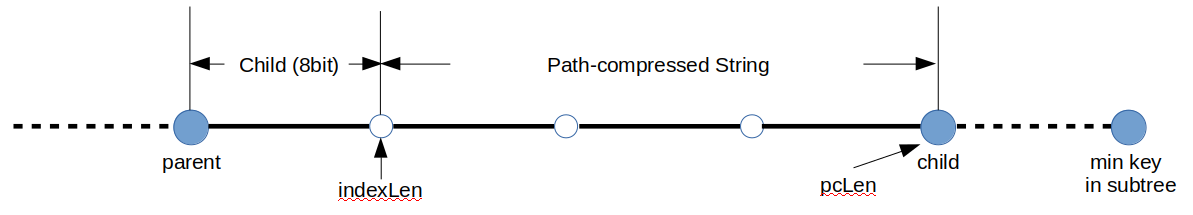
\includegraphics[width=\linewidth]{mlpindex64_node.png}
\caption{The trie node structure for $\MlpIndex$ on 64-bit keys.}
\label{mlpindex64_node}
\end{figure}

One note that the ``index'' and the ``prefix including path-compressed string'' is always a prefix of the minKey, 
so we only need to store the minKey as well as the lengths. 
For 64-bit keys, we need around 12 bytes to store the necessary information of a trie node, 
as shown in the following memory layout:

\singlespacing\begin{codebox}
\begin{minted}{c++}
// the layout of a hash table entry (which is also a trie node)
struct Node {
    // whether this hash table slot is occupied
    uint32_t occupyFlag:2; 
    // length of this node in bytes in the trie
    uint32_t indexLen:3;
    // length of this node plus its path-compressed string
    uint32_t pcLen:3;
    // hash fingerprint, length adjustable but needs some bits
    uint32_t hash:18;
    // the minKey in this subtree
    // the first indexLen bytes is the prefix of this node in trie
    // the first pcLen bytes is the prefix + path-compress string
    uint64_t minKey;
};  
\end{minted}
\end{codebox}\doublespacing

So always spending 32 bytes to store a bitmap seems too much a waste. 
Instead, we will always have slots of size 24 bytes, 
and ``small nodes'' which occupies one slot, and ``large nodes'' which occupies 2 slots. 
It is possible to have finer-grained node sizes, as discussed in paragraph \ref{variantsizehash}, 
but for now we only consider two node sizes for ease of understanding and implementation.

Small nodes are nodes with no more than 8 children.
We spend a byte to store the number of children in this node, 
and store the children as a list, each taking one byte. 
Large nodes are nodes with at least 8 children. 
The children are stored as a bitmap of 32 bytes, as described before.

The tricky thing is, how could we arrange nodes of different sizes in the same hash table?
Using pointer indirection is not a solution, since we don't want to incur additional cache miss. 
Another good property of cuckoo hashing comes in: 
unlike other closed-addressing schemes that may have ``clusters'' of occupied slots, 
the possibility of each slot is occupied in cuckoo hash table is independent, 
and simply equals the load factor. 
So we can ``steal'' an unused slot from the neighborhood of the slot for the ``big node'' to form a 48-byte node. 
That unused slot should reside in the same 128-byte line,
so the hardware adjacent-line prefetcher described in Section \ref{adjlineprefetcher} can take advantage.
Since the load factor is at most 50\% and there are 4 possible slots (since a 128-byte line holds 5 slots) to steal from, 
with probability at least $15/16$ we can find such an empty slot. If not, we fall back to the pointer-indirection solution
by allocating a piece of external memory and store the pointer in the hash table. 
When a cuckoo replacement sequence wants to evict a ``stolen slot'', one can know that it is a stolen slot 
from its occupyFlag, and ask its owner to steal another slot instead (or fall back to pointer indirection) to make this slot free.  
When the ``main node'' itself is evicted by cuckoo replacement, it frees the slot it stole, 
and steals another slot (or fall back to pointer indirection) near the slot it is moved to.
 
Each big node of degree $\geq 8$ consumes 48 bytes of memory, but the total number of ``degrees'' in the trie is fixed 
-- it is always the number of nodes in the trie tree minus 1, which is no larger than $2n-1$. 
Since $48/8<24/2$, memory usage is peaked when all nodes are small nodes, 
and the total memory used by the data structure is bounded by 24 bytes times $2n$ nodes over 50\% load factor, 
which is 96 bytes per 8-byte key.

\subsubsection*{Bucketized Cuckoo Hashing}  \label{variantsizehash}

We may combine the idea of adaptive node size with bucketized cuckoo hashing for even reduced memory consumption. 
We will have a bucket size of 4 and a hash table entry size of 16 bytes (so each bucket of entries consumes exactly one cache line).
We will have 3 types of nodes: small node, medium node and large node, consuming 16, 32, 48 bytes each. 
As before, small node and medium node stores children directly, and will hold at most 3 / 16 children. 
Large node stores children in a bitmap. A node must reside in the same bucket of entries, 
so a large node needs to consume 3 slots in the bucket, etc.

The variant-sized nodes makes Cuckoo replacement a little different. 
Specifically, we may have to reserve multiple slots of space to insert a large node, 
and evict multiple elements in the process. 
This makes the theoretical analysis of Cuckoo hashing no longer working. 
However, since at most $1/4$ of the nodes are medium nodes 
and at most $1/17$ portion of nodes are large nodes, 
intuitively it should not have too much effect on the maximum load factor. 
Indeed, experiments show that one can still reach at least 90\% load factor with various combinations 
of medium/large node percentage.

By averaging the size of the node over the minimum degrees, 
one can see that memory usage is still peaked when all nodes are small nodes.
So now, the total memory usage is bounded by 16 bytes times $2n$ nodes over 90\% load factor, 
which is around 36 bytes per 8-byte key.

However, due to time limitation, we are unable to implement this bucketized cuckoo scheme 
into $\MlpIndex$. All evaluations in Section \ref{mlpindex_eval} are done using the 96-byte-per-key version. 

\subsubsection*{Flat Bitmap For Top Layers of Trie Tree}

This is an extra optimization for 64-bit keys.
The top two layers of the trie tree can only hold $256^3$ different children. 
It would additionally save some space, as well as DRAM accesses, to simply store the first 2 layers
in a flat array, each using a bitmap of 256 bits (32 bytes) to store which children exists. 
This results in a bitmap of $256^2\times 32$ bytes ($2MB$), instead of the hash table. 
After this optimization, we only need to access 6 layers times 2 (per cuckoo lookup) plus 1 (the top-layers bitmap), 
which is 13 DRAM positions in parallel, to execute a $\QueryLCP$ for 64-bit keys, 
which is another small performance and memory-consumption improvement.
 
\subsubsection*{The Choice of Hash Function}

Finally, we need a good hash function family.
The hash functions should be very efficient to compute (so it doesn't drag our performance down), 
vectorizable (since we need to compute multiple independent strings' hash value) 
and have high quality (required for cuckoo hash scheme to reach its theoretical maximum load factor).
While there may definitely be other choices that meet the criteria, 
we chose xxHash \cite{xxhash}, 
a hash function family widely used in industry that is both extremely preferment and of high quality.

\subsection{Evaluation} \label{mlpindex_eval}

In this section, we benchmark $\MlpIndex$ on 64-bit keys against other state-of-the-art data structures. 
The hardware setting is Intel Core i7-7700HQ CPU at 2.80GHz and 2x16GB Corsair DDR4 2400MT DRAM.

\subsubsection*{Benchmark Rivals}

We benchmarked $\MlpIndex$ against two fastest ordered index 
structures to the best of our knowledge -- the Height Optimized Trie (HOT) \cite{hot_sigmod18} and the Adaptive Radix Tree (ART) \cite{arttrie_icde13}.
We also benchmark against
a widely-used hash table \cite{densehashset} and a carefully-engineered binary search algorithm (EBS \cite{binary_search_layout}), 
two well-known methods that can only support a subset of the ordered index operations. 
Since they are designed to specialize on a certain type of operation, 
it demonstrates the cost we took to support all operations simultaneously. 
The details of our benchmark rivals can be find below:
\begin{itemize}
[topsep=0pt,partopsep=0pt,itemsep=0pt,parsep=0pt,fullwidth,itemindent=\parindent,listparindent=\parindent]
\item \textit{HashTable}: a hash table supports $\insertion$ and $\lookup$ in $O(1)$ expected time, but cannot support $\lowerbound$ queries.
We used Google's dense\_hash\_set \cite{densehashset},
a quadratic probing hash table scheme widely used in industry.
The effective load factor of the dense\_hash\_set is 60\%, 
though the performance is almost the same with a effective load factor of 30\%.
We resized the table at the beginning to prevent resize cost due to table overflow.
\item \textit{EBS} \cite{binary_search_layout}: short for ``B-tree-like multi-way Search on Eytzinger-layout static array''. 
As the name suggests, it is a carefully engineered binary search on a static data set, 
so it supports $\lowerbound$ but not $\insertion$.
The authors of \cite{binary_search_layout} concluded that this is the fastest binary search algorithm on large data sets 
amongst a variety of binary search algorithm variants they investigated. 
We used the variant that is empirically fastest on our machine, which uses 16-way implicit B-tree Eytzinger layout
+ ``low-level optimizations such as unrolling and conditional moves''
(the ``btree16\_a'' variant in authors' benchmark). 
EBS is around 2x faster than the straightforward approach of invoking std::lower\_bound on a sorted array.
\item \textit{HOT} \cite{hot_sigmod18}: this is the fastest ordered index structure to the best of our knowledge. 
We use the public-available implementation released along with the original paper.
We believe we configured the library correctly,
as the numbers we get generally match what are demonstrated in the original paper (it is slightly slower 
because we are using a larger data set, and our CPU frequency is slower than the CPU in their paper).
\item \textit{ART} \cite{arttrie_icde13}: this was the fastest ordered index structure we are aware of, before HOT was published.
We use the public-available implementation released along with the original paper.
It is a single-file library so there is no potential configuration issue.
We note that while ART could support $\lowerbound$ queries, 
the public-available implementation only supports prefix-search, 
which is more restrictive than general $\lowerbound$. 
As such we are unable to test the $\lowerbound$ performance for ART.
\end{itemize}

We did not benchmark against comparison-based data structures such as the B-tree variants 
(STX B-tree \cite{stx_btree}, FAST \cite{fast_sigmod10}, etc), 
or Masstree \cite{masstree} (a B-tree/trie-tree hybrid data structure),
since they are much slower on 64-bit keys than HOT and ART, as shown in both papers \cite{hot_sigmod18, arttrie_icde13}.
Everything is single-threaded in the benchmark, and 1GB huge page is used for $\MlpIndex$, EBS and dense\_hash\_set. 
Our implementation of $\MlpIndex$ is available at \cite{mlpds_repo}.

Finally, we also ``benchmark'' $\MlpIndex$ against itself, 
by comparing $\MlpIndex$'s ``theoretical'' performance derived from the models built in Section \ref{understandmlp} 
with its practical performance. 

\subsubsection*{Data Distribution and Configuration}

We use a family of data distribution similar to the ones used in \cite{masstree}, which \cite{masstree} calls ``decimal distribution''. 
In this distribution, we generate the key byte by byte, and each byte is randomly selected from a set of candidates, 
which may vary depending on the position of this byte in the key.
The trie tree built from this distribution has both high-degree and low-degree nodes, 
and while path compression can help lower the height of the trie, it will not ``collapse'' the trie 
to essentially a big flat array like the uniform random distribution would. 
As such, we believe this distribution family is a balanced test that 
benchmarks multiple components of trie-based data structures and does not over-emphasize a particular component. 

Due to time limitation, we only tested two such distributions. 
In distribution $A$, the first (higher-ordered) 6 bytes have a small candidate set of 6 elements for each byte, 
and the last 2 bytes have a large candidate set of around 100 elements. 
Distribution $B$ is mirror to $A$: the first 2 bytes have a large candidate set of around 100 elements,
while the last 6 bytes have a small candidate set of 6 elements for each byte.
Both data set contains 80 million elements.

$\lookup$ queries are generated as a mix of keys sampled directly from the data set (so the $\lookup$ must yield positive result),
and keys sampled from the same distribution that generated the data set (so it exists in the original data set 
with only a small probability). The final positive rate for $\lookup$ is controlled to be around 80\%. 
Keys for $\lowerbound$ queries are generated using the same distribution as the original data set is generated. 
About 15\% of the $\lowerbound$ query keys appeared in original data set, the remaining 85\% do not. 

In order to more accurately measure the time needed to execute one operation, 
we want to make sure that each query is indeed executed ``independently'', 
so the total time over total number of queries indeed reflects what it takes to execute one query. 
To see what it means, we will use the cuckoo hash table as an example. 
Recall that each cuckoo hash lookup looks like this:

\singlespacing\begin{codebox}
\begin{minted}{c++}
bool Lookup(Key x) {
    uint32_t hash1 = HashFn1(x), hash2 = HashFn2(x);
    return table[hash1].key == x || table[hash2].key == x;
}
\end{minted}
\end{codebox}\doublespacing

If one simply write the following code to benchmark the time needed per lookup, 
one will unfortunately get deceptive results.

\singlespacing\begin{codebox}
\begin{minted}{c++}
// A bad way to benchmark the performance of "Lookup" above
START_TIMING();
for (int i = 0; i < N; i++) { 
    result[i] = Lookup(data[i]);
}
END_TIMING();
\end{minted}
\end{codebox}\doublespacing

Not only the compiler will unroll the loop and arbitrarily interleave the instructions, 
the CPU's out-of-order execution mechanism will do it as well. 
While it is unlikely for the CPU and compiler to take this advantage in real-world applications, 
since there are likely a lot of application logic and data dependencies between two hash table queries, 
they will take this advantage in this tight and logic-less benchmark loop, and give out deceptive results. 
The solution is to use the same trick as in Section \ref{understandmlp}. 
We will hide the query text from compiler reordering and CPU out-of-order and speculative execution by 
XORing it with the correct answer to the previous query. 
Now the CPU cannot know what the next query is until it completes the execution of the previous one and yield the answer, 
thus ``total time over total number of query'' actually represents the time to execute one query. 
This results in a code like this:

\singlespacing\begin{codebox}
\begin{minted}{c++}
// "Encrypt" query input with the 
// expected result of the previous query
for (int i = 1; i < N; i++) {
    data[i] ^= expected_result[i-1];
}
// benchmark loop
START_TIMING();
uint64_t lastAnswer = 0;
for (int i = 0; i < N; i++) { 
    // "Decrypt" query input by the correct 
    // answer to the previous query 
    uint64_t realInput = data[i] ^ lastAnswer;
    lastAnswer = Lookup(realInput);
    result[i] = lastAnswer;
}
END_TIMING();
\end{minted}
\end{codebox}\doublespacing

We note that this ``query encryption'' only make significant (1.5x to 2x) difference on hash table, mainly due to its extremely simple logic. 
For ordered index, all benchmarked implementation, including $\MlpIndex$, becomes slower, but only by a small degree (less than 10\%). 
This is as expected: since CPU speculative execution only have a small window, it is unsurprising that it 
cannot penetrate complicated logic effectively. 

\subsubsection*{Benchmark Results}

The benchmark results on data distribution $A$ and $B$ can be found in Figure \ref{mlpindex_distA} and \ref{mlpindex_distB} respectively.
Raw numbers can be found in Table \ref{mlpindex_results}.

\begin{figure}[!htb]
\centering
  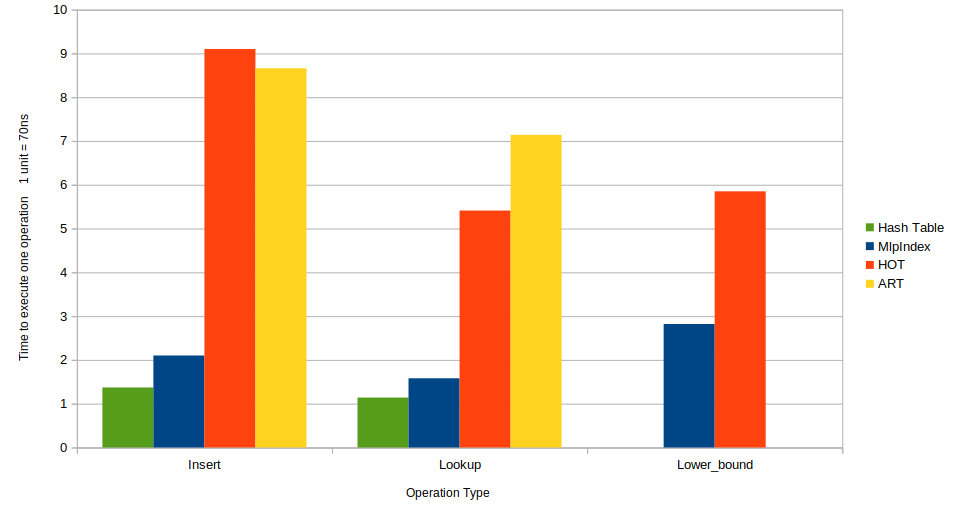
\includegraphics[width=0.8\linewidth]{mlpindex_result1.png}
\caption{Data distribution A (80 million 64-bit keys). Comparison on time to execute one operation. 
Each unit of Y-axis represent 70ns, which is 1 DRAM roundtrip time on the machine running the benchmark.}
\label{mlpindex_distA}
\end{figure}

\begin{figure}[!htb]
\centering
  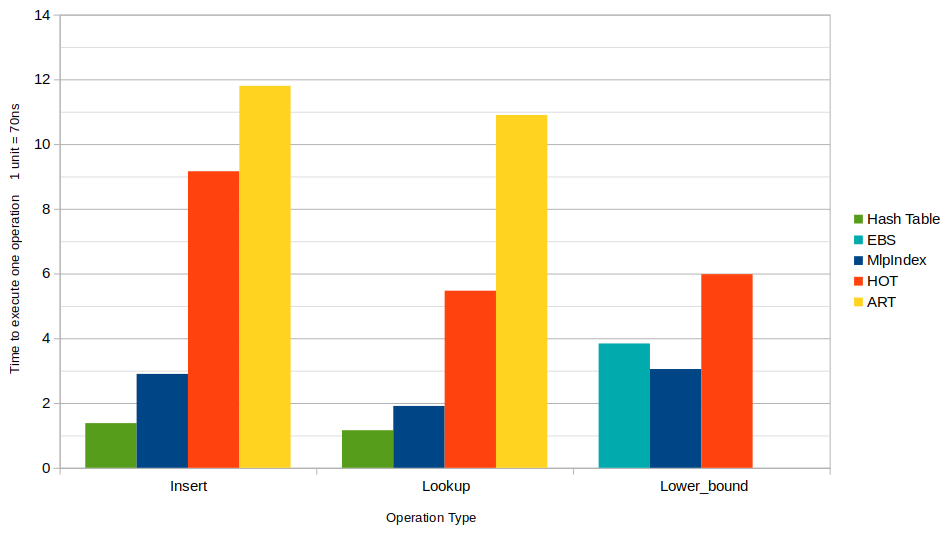
\includegraphics[width=0.8\linewidth]{mlpindex_result2.png}
\caption{Data distribution B (80 million 64-bit keys). Comparison on time to execute one operation. 
Each unit of Y-axis represent 70ns, which is 1 DRAM roundtrip time on the machine running the benchmark.}
\label{mlpindex_distB}
\end{figure}

As one can see, $\MlpIndex$, despite being an ordered index, 
has a performance competitive with a well-engineered hash table on $\insertion$ and $\lookup$, 
and its $\lowerbound$ performance is even better than EBS, 
the extensively optimized static-data-set binary search designed to specialize at $\lowerbound$.
On data distribution $A$, we only take 1.5x and 1.4x the time of the hash table respectively, to do an $\insertion$ and $\lookup$. 
On distribution $B$ our performance is slightly worse: 2.1x and 1.7x respectively. 
But still, when compared with state-of-the-art ordered index structures, 
on distribution $A$, we are 4.3x faster than HOT and ART on $\insertion$, 
3.5x faster than HOT and 4.5x faster than ART on $\lookup$, 
and more than 2x faster than HOT on $\lowerbound$. 
On distribution $B$, we are 3.1x faster than HOT, 4x faster than ART on $\insertion$, 
2.8x faster than HOT, 5.6x faster than ART on $\lookup$, 
and 2x faster than HOT on $\lowerbound$.

The comparison between $\MlpIndex$ and EBS is especially interesting. 
It may look surprising at first glance: how could it be possible for one to support fast insertions, 
while simultaneously having a faster lookup than a data structure specially designed for static data sets?
Plus that, the EBS authors also carefully engineered their memory layouts 
to optimize the cache efficiency, as well as used a B-tree-like structure to decrease the length of the search.
The key comes in two points. First, we are an integer data structure, while EBS is a comparison-based data structure. 
This allows us to achieve theoretically better complexity, specifically, $O(\log\log M)$ versus $O(\log n)$. 
Second, our design allows us to effectively leverage MLP to further shorten the DRAM dependency chain, 
while EBS, essentially a carefully-layouted B-tree, cannot effectively leverage MLP. 
All it can do is move down the tree level by level, resulting in a longer DRAM dependency chain than us. 
Despite that the static tree layout allows one to know the address of the children nodes without having 
the parent node fetched into memory, 
the best one can do to ``look-ahead'' one level is still to prefetch all the $B$ children of a B-tree node, 
which turns out to be too costly. Indeed, the experiments in the authors' repository 
showed that prefetching only slows things down for all ``B-tree Eytzinger'' category algorithms.
But why is the performance difference between $\MlpIndex$ and EBS not so large? 
The main reason is, EBS has an important advantage that we don't: it can leverage cache hierarchy much better than us. 
Specifically, the top of its B-tree will be cache-resident, 
so despite that it has a longer DRAM dependency chain, many accesses at the beginning of the chain will hit L1/L2/L3 
cache, making them cheaper (to a varied degree) than a real DRAM access. 
However, this is not the case for us. We issue $D$ independent accesses in parallel, 
and clearly not all of them are cache resident, so cache effect has little help for us.
However, we note that since the cache has a fixed size, we would have larger advantage on larger data sets; 
and while in benchmark one can exclusively own all the caches, it is impractical to assume so in real world settings,
as all the other components in a real application will use cache space as well. 
So the fact that our performance does not rely much on L2/L3 cache is actually an advantage in real world.

$\MlpIndex$, from algorithm level, is not input-data dependent. 
Indeed, for 64-bit keys, all we do is going through a series of parallel hash table lookup, 
then additionally do hash table insertion for $\insertion$, or an additional hash table lookup for $\lowerbound$. 
Why is it slower on Distribution $B$ than Distribution $A$? 
We believe the most important reason is that Distribution $A$ has high-degree nodes at the bottom levels, 
which makes the LCP likely to be found at deeper levels of the trie. 
When we do the parallel hash table lookups, we checked the results in reverse order of depth, 
so we can quit whenever a hit is found. 
So on Distribution $A$ we are likely to exit earlier than Distribution $B$ when finding LCP, 
resulting in an effectively smaller number of DRAM requests issued 
(despite that all prefetches have been issued at the beginning, if a prefetched address is not actually used, 
the latency of this prefetch is shadowed in the background because it does not affect the critical path), 
making it faster.

To better understand the performance, 
we compare the ``theoretical'' performance derived from the models in Section \ref{understandmlp} against the real performance. 
Note that in the ``theoretical'' model, 
we treated all CPU work and cache-hitting DRAM accesses as free (or can be completely shadowed by cache misses) 
and only consider the DRAM latency.

Recall that for 64-bit keys, we make at most 13 independent DRAM accesses to perform a $\QueryLCP$ operation. 
Plugging in the empirical formula in Section \ref{mlpmeasurement}, it should take around $2.4$ DRAM roundtrip time.
All a $\lookup$ does is checking the result of $\QueryLCP$, so 2.4 is the ``theoretical cost'' for $\lookup$. 
For $\insertion$, if there is no hash table movement due to conflict, we will only write addresses that are cache-resident, 
which are also considered free in our model. 
By collecting statistics, we observed that the average length of cuckoo replacement chain is around 0.5 per $\insertion$. 
So $\insertion$ should have a ``theoretical cost'' of 2.9.
For $\lowerbound$, we always spend an additional DRAM request, 
so it has a ``theoretical cost'' of 3.4. We compare the above theoretical cost with the practical time 
on the two data distributions in Table \ref{mlpindex_theory_practice}.

\begin{table}[]
\centering
\begin{tabular}{|c|c|c|c|}
\hline
                             & Theory                      & Dist A                      & Dist B                      \\ \hline
$\lookup$                      & 2.4                         & 1.58                        & 1.91                        \\ \hline
\multirow{2}{*}{$\insertion$}  & 2.9                         & 2.10                        & 2.90                        \\ \cline{2-4} 
                             & L+0.5                      & L+0.52                      & L+0.99                      \\ \hline
\multirow{2}{*}{$\lowerbound$} & 3.4                         & 2.82                        & 3.05                        \\ \cline{2-4} 
                             & \multicolumn{1}{c|}{L+1} & \multicolumn{1}{c|}{L+1.22} & \multicolumn{1}{c|}{L+1.14} \\ \hline
\end{tabular}
\caption{Theoretical (worst case spent in DRAM latency) and practical time for $\MlpIndex$ to execute one operation, in DRAM roundtrip time.
Insertion cost is amortized. $L$ represent the time for $\lookup$ in respective column.}
\label{mlpindex_theory_practice}
\end{table}

The ``base'' difference, i.e. the time needed to execute one $\QueryLCP$ or one $\lookup$, 
is already explained by difference in average depth of the LCP node, which varies according to data set. 
So now we will focus on the delta between $\insertion$ / $\lowerbound$ operation and $\lookup$ operation.

In the theory model, $\lowerbound$ should take 1 more DRAM roundtrip time than $\lookup$; 
but in practice it takes around 1.2 more DRAM roundtrip time. 
We believe the extra time is spent in finding the minimum child that is larger than the given one in the 256 fan-outs of the LCP trie node. 
We used multiple (cache-hitting) memory requests, SIMD operations and branches in the logic, 
which, despite much faster than a cache miss, still requires non-negligible CPU time.

$\insertion$ involves non-negligible work to insert new nodes into hash table and update the extra-information fields along the path. 
We note that the total number of nodes in the trie tree in distribution $A$ is smaller than that in distribution $B$, 
since distribution $A$ has much more high degree nodes than distribution $B$ does.
This results in less CPU work and less cuckoo hash displacements, which we believe is the reason that $\insertion$ is faster on distribution $A$.

\begin{table}[!htb]
\centering
\begin{tabular}{|c|c|c|c|c|c|c|}
\hline
\multirow{2}{*}{} & \multicolumn{3}{c|}{Data Distribution A} & \multicolumn{3}{c|}{Data Distribution B} \\ \cline{2-7} 
                                                                             & \ $\insertion\ $   & \ $\lookup\ $   & $\lowerbound$   & \ $\insertion\ $   & \ $\lookup\ $   & $\lowerbound$   \\ \hline
Hash Table                                                                    & 10.44        & 12.50     & N/A           & 10.37        & 12.34     & N/A           \\ \hline
EBS                                                                          & N/A          & 3.72     & 3.70           & N/A          & 3.74      & 3.72           \\ \hline
$\MlpIndex$                                                                    & 6.80         & 9.03      & 5.06          & 4.93         & 7.40      & 4.69          \\ \hline
HOT                                                                          & 1.57         & 2.64      & 2.44          & 1.56         & 2.61      & 2.39          \\ \hline
ART                                                                          & 1.65         & 2.00      & N/A           & 1.21         & 1.31      & N/A           \\ \hline
std::set                                                                     & 0.71         & 0.67      & 0.67           & 0.73        & 0.67      & 0.67           \\ \hline
\end{tabular}
\caption{Raw throughput numbers in million operations per second.}
\label{mlpindex_results}
\end{table}

\section{Future Work} \label{futureworks}

In this section, we briefly mention a few possible directions of future works. 

While our skiplist iterator works seamlessly for lock-free skiplist, 
$\MlpIndex$ is currently single-threaded only. 
It would be interesting to support a multi-threaded version of $\MlpIndex$.
What would be the best locking protocol for $\MlpIndex$? 
Would it be fine-grained locking, read-optimized-write-exclusive locking, or even lock-free?
How well would $\MlpIndex$ perform in multi-threaded scenario, 
compared with other multi-threaded index structures, such as ROWEX ART \cite{art_sync}, Masstree \cite{masstree},
lock-free skiplist \cite{lockfree_skiplist}, or Bw-Tree \cite{bwtree}?

Currently we only support 64-bit keys for $\MlpIndex$. 
So another direction of work is to support general string keys. 
For $\MlpIndex$, we will eventually need more than 2 layers of data structures, 
for sufficiently long key. But what length is the correct breaking point?
What is the best ``query execution plan'' for each key length?
For longer string keys, a lot of our sub-data-structures will only be managing a small set of keys. 
What will be the best data structure to manage data of each magnitude? 
How well would our data structure perform compared with HOT and ART, 
as well as string-key-oriented data structure such as Masstree?
Even more, would it be possible to combine string support and multi-threading support?
Would it be possible to add transactional support or snapshotting and make it a 
real-world database engine? 

The developments in hardware is also posing new challenges to memory level parallelism, 
for example, Intel is planning to publish the non-volatile DIMM memory in 2019.
Persistable through power-offs and byte-addressable, 
although each access has a much higher latency than current memory chips. 
Would it be possible to develop data structures that leverages memory level parallelism 
on those new hardware to mitigate the high latency? 

\section{Conclusion} \label{conclusion}

In this paper, we demonstrated that data structures that are designed to leverage high memory level parallelism 
can achieve the performance not considered possible before, 
typically a few times faster than the current state-of-the-arts. 

\section*{Acknowledgments}

I am grateful to my mentor Vladimir Kiriansky for his extensive help and discussions throughout the research 
and the writing of this paper. Thanks Saman Amarasinghe, Yinzhan Xu and Martin Rinard for the review and advice on writing the paper. 
Thanks MemSQL Inc. for providing the opportunity to evaluate my skiplist iterator in a real database, 
as well as their CTO Drew Paroski, for the permission to release my findings to public.

\bibliography{ref}{}
\bibliographystyle{plain}

\end{document}



%%  LocalWords:  Haoran Xu Amarasinghe Rinard CPUs roundtrip MLP APIs
%%  LocalWords:  pipelining skiplist microarchitecture SIMD ns Epyc
%%  LocalWords:  clockrate prefetcher Skylake prefetch analytics AMAC
%%  LocalWords:  prefetching lookups prefetches unmaintainable MemSQL
%%  LocalWords:  coroutine codebase trie roundtrips EBS ytzinger DDR
%%  LocalWords:  earch Haswell struct uint idx branchy newIndex TLB
%%  LocalWords:  oldSum th NUMA dereference PayloadType prefetched nL
%%  LocalWords:  QueueItem enqueue ProcessQueueItem ProcessQueue sql
%%  LocalWords:  newQueue pseudocode const benchmarked lockfree Radix
%%  LocalWords:  SingleBox sharding vectorized adaptively Redis Prev
%%  LocalWords:  Masstree subtree Succ prev succ IsLeaf nullptr LCP
%%  LocalWords:  len QueryLCP logM bool newNode hashTable MLPIndex DS
%%  LocalWords:  UpdateFields ary fullKey isSpecialIntermediateNode
%%  LocalWords:  recurse currentDepth lcp lcpNode substring Emde STX
%%  LocalWords:  prefixToFind fullKeyLen isAllSmallerThanKey amongst
%%  LocalWords:  bucketized minKey occupyFlag indexLen pcLen xxHash
%%  LocalWords:  vectorizable Eytzinger btree HashFn XORing Decrypt
%%  LocalWords:  lastAnswer realInput layouted ROWEX Bw transactional
%%  LocalWords:  snapshotting DIMM Persistable Yinzhan CTO Paroski
